\clearpage
\section{Anhang}
\begin{figure}[h]
\begin{center}
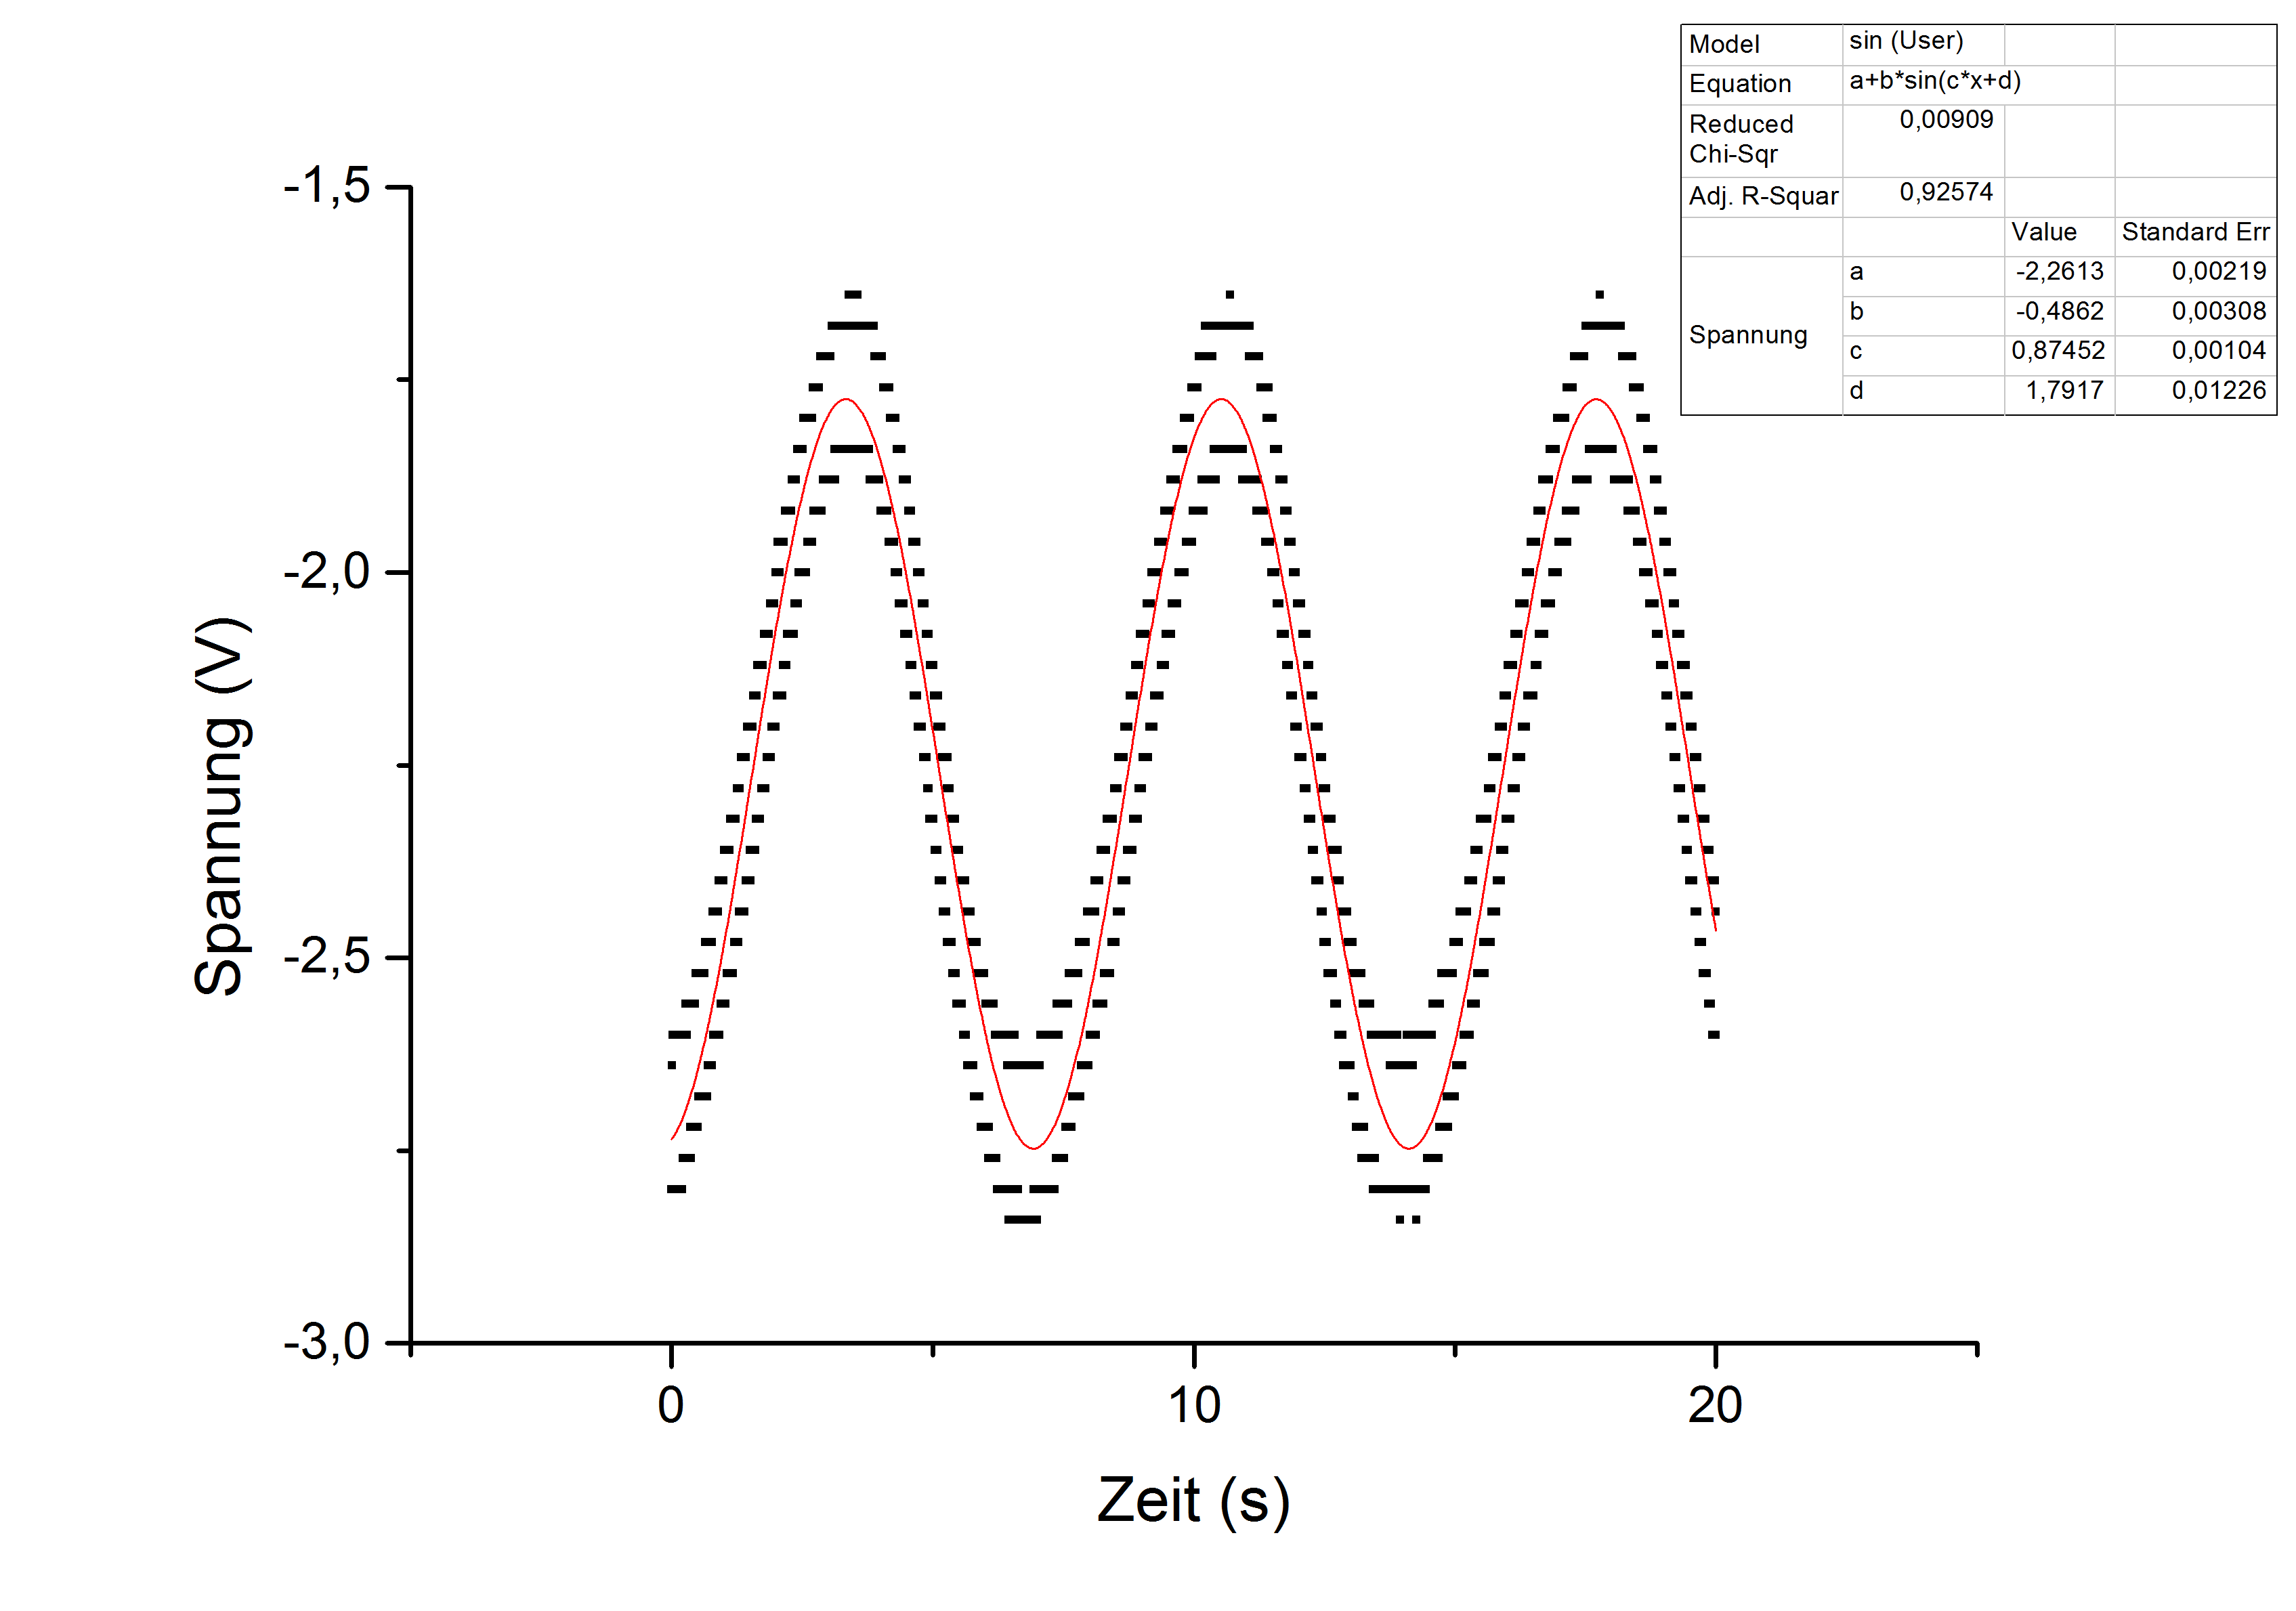
\includegraphics[scale=0.6]{Bilder/w1}
\caption{Messung mit Widerstand R1}
\end{center}
\end{figure}
\begin{figure}[h]
\begin{center}
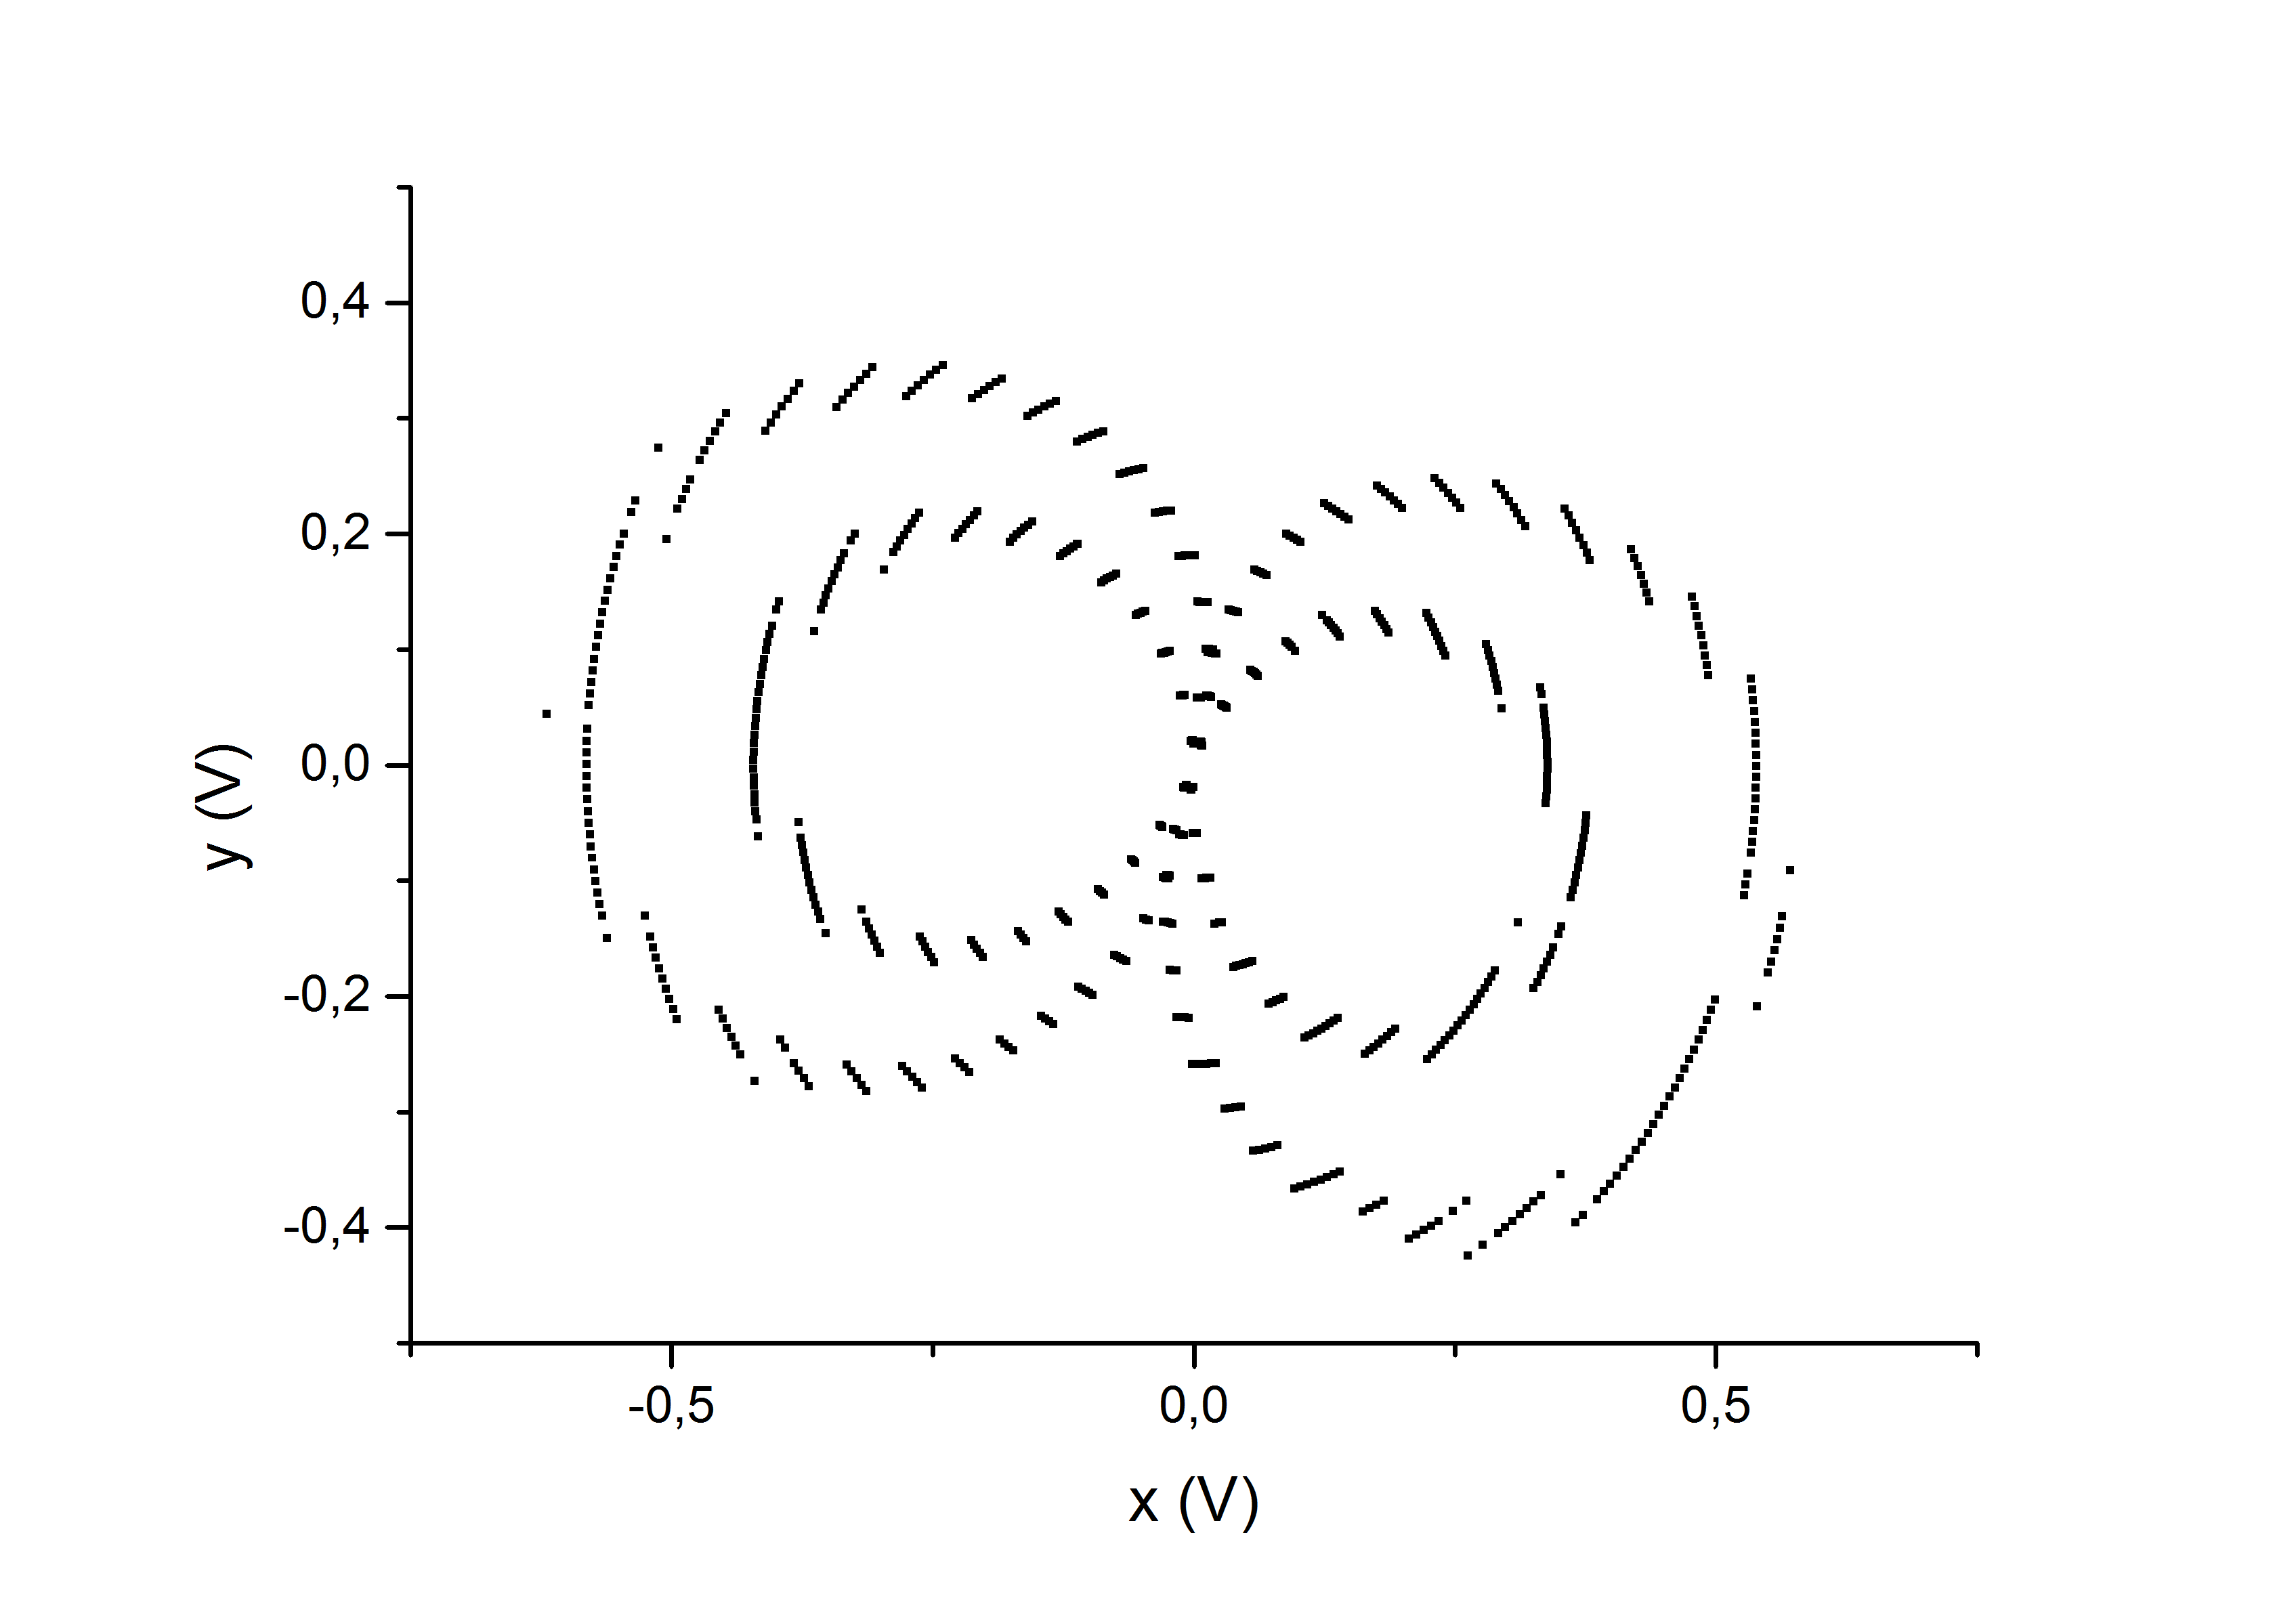
\includegraphics[scale=0.6]{Bilder/pw1}
\caption{Polarplot mit Widerstand R1}
\end{center}
\end{figure}
\begin{figure}[h]
\begin{center}
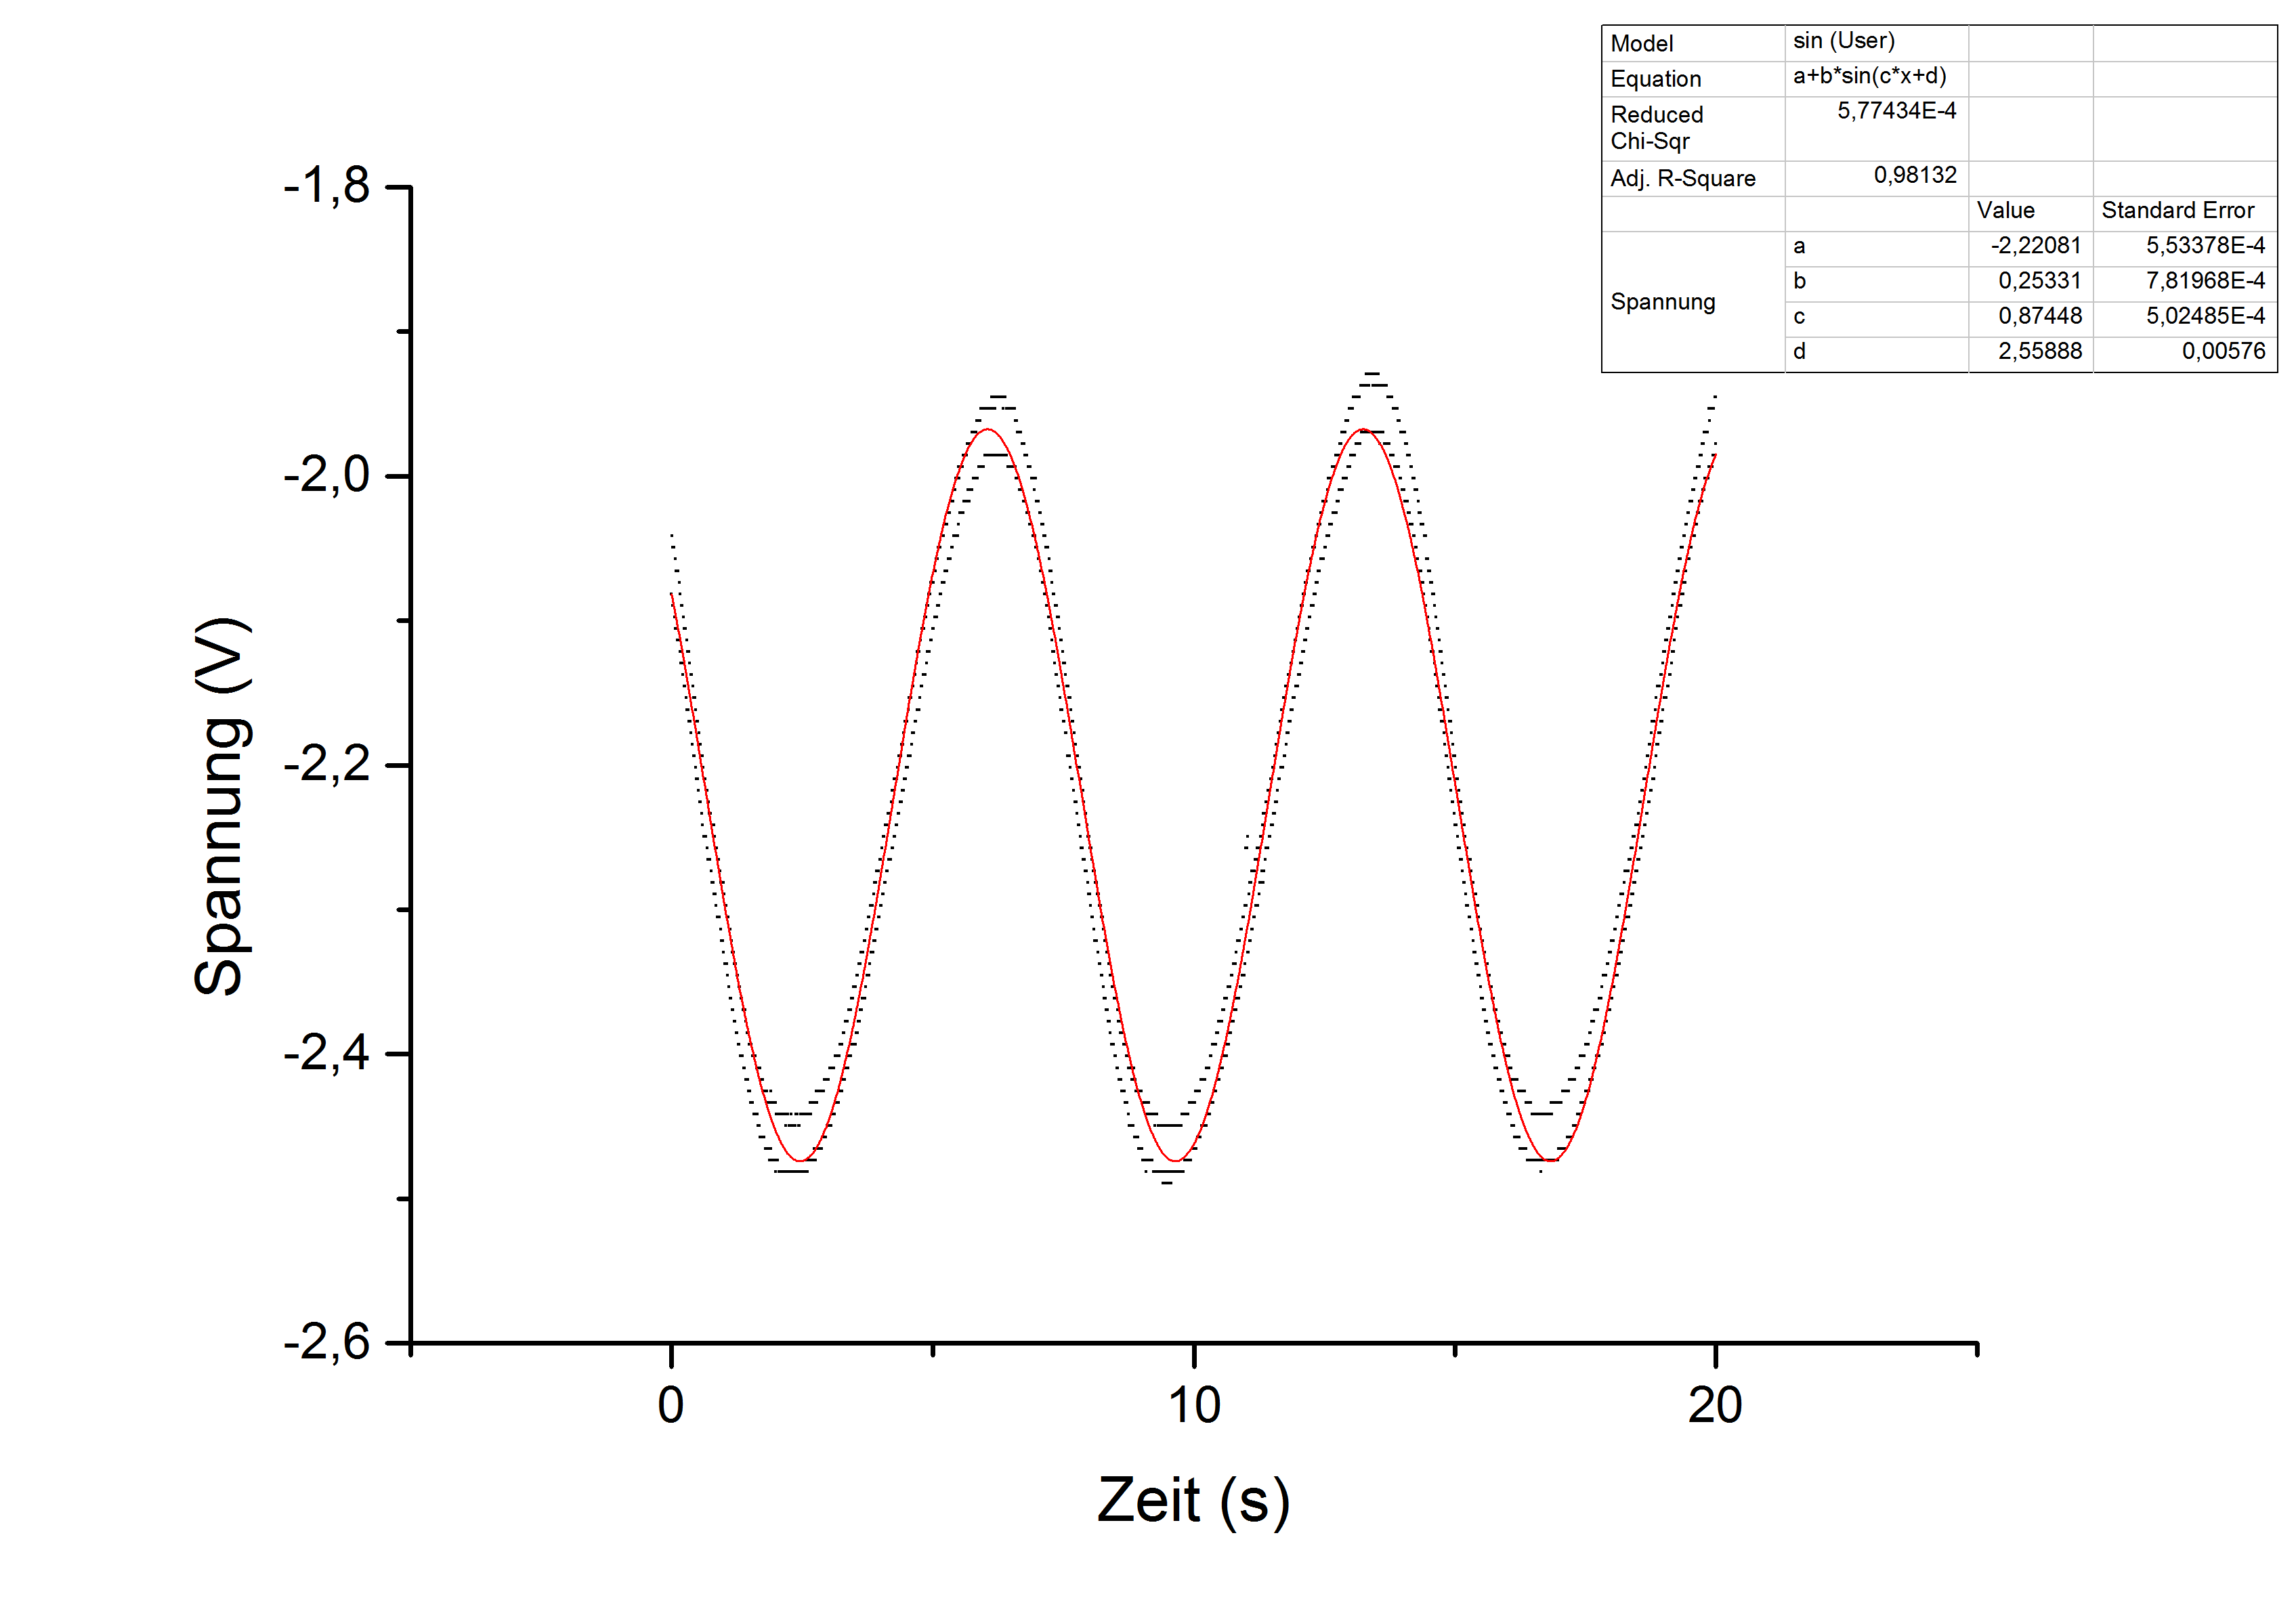
\includegraphics[scale=0.6]{Bilder/w2}
\caption{Messung mit Widerstand R2}
\end{center}
\end{figure}
\begin{figure}[h]
\begin{center}
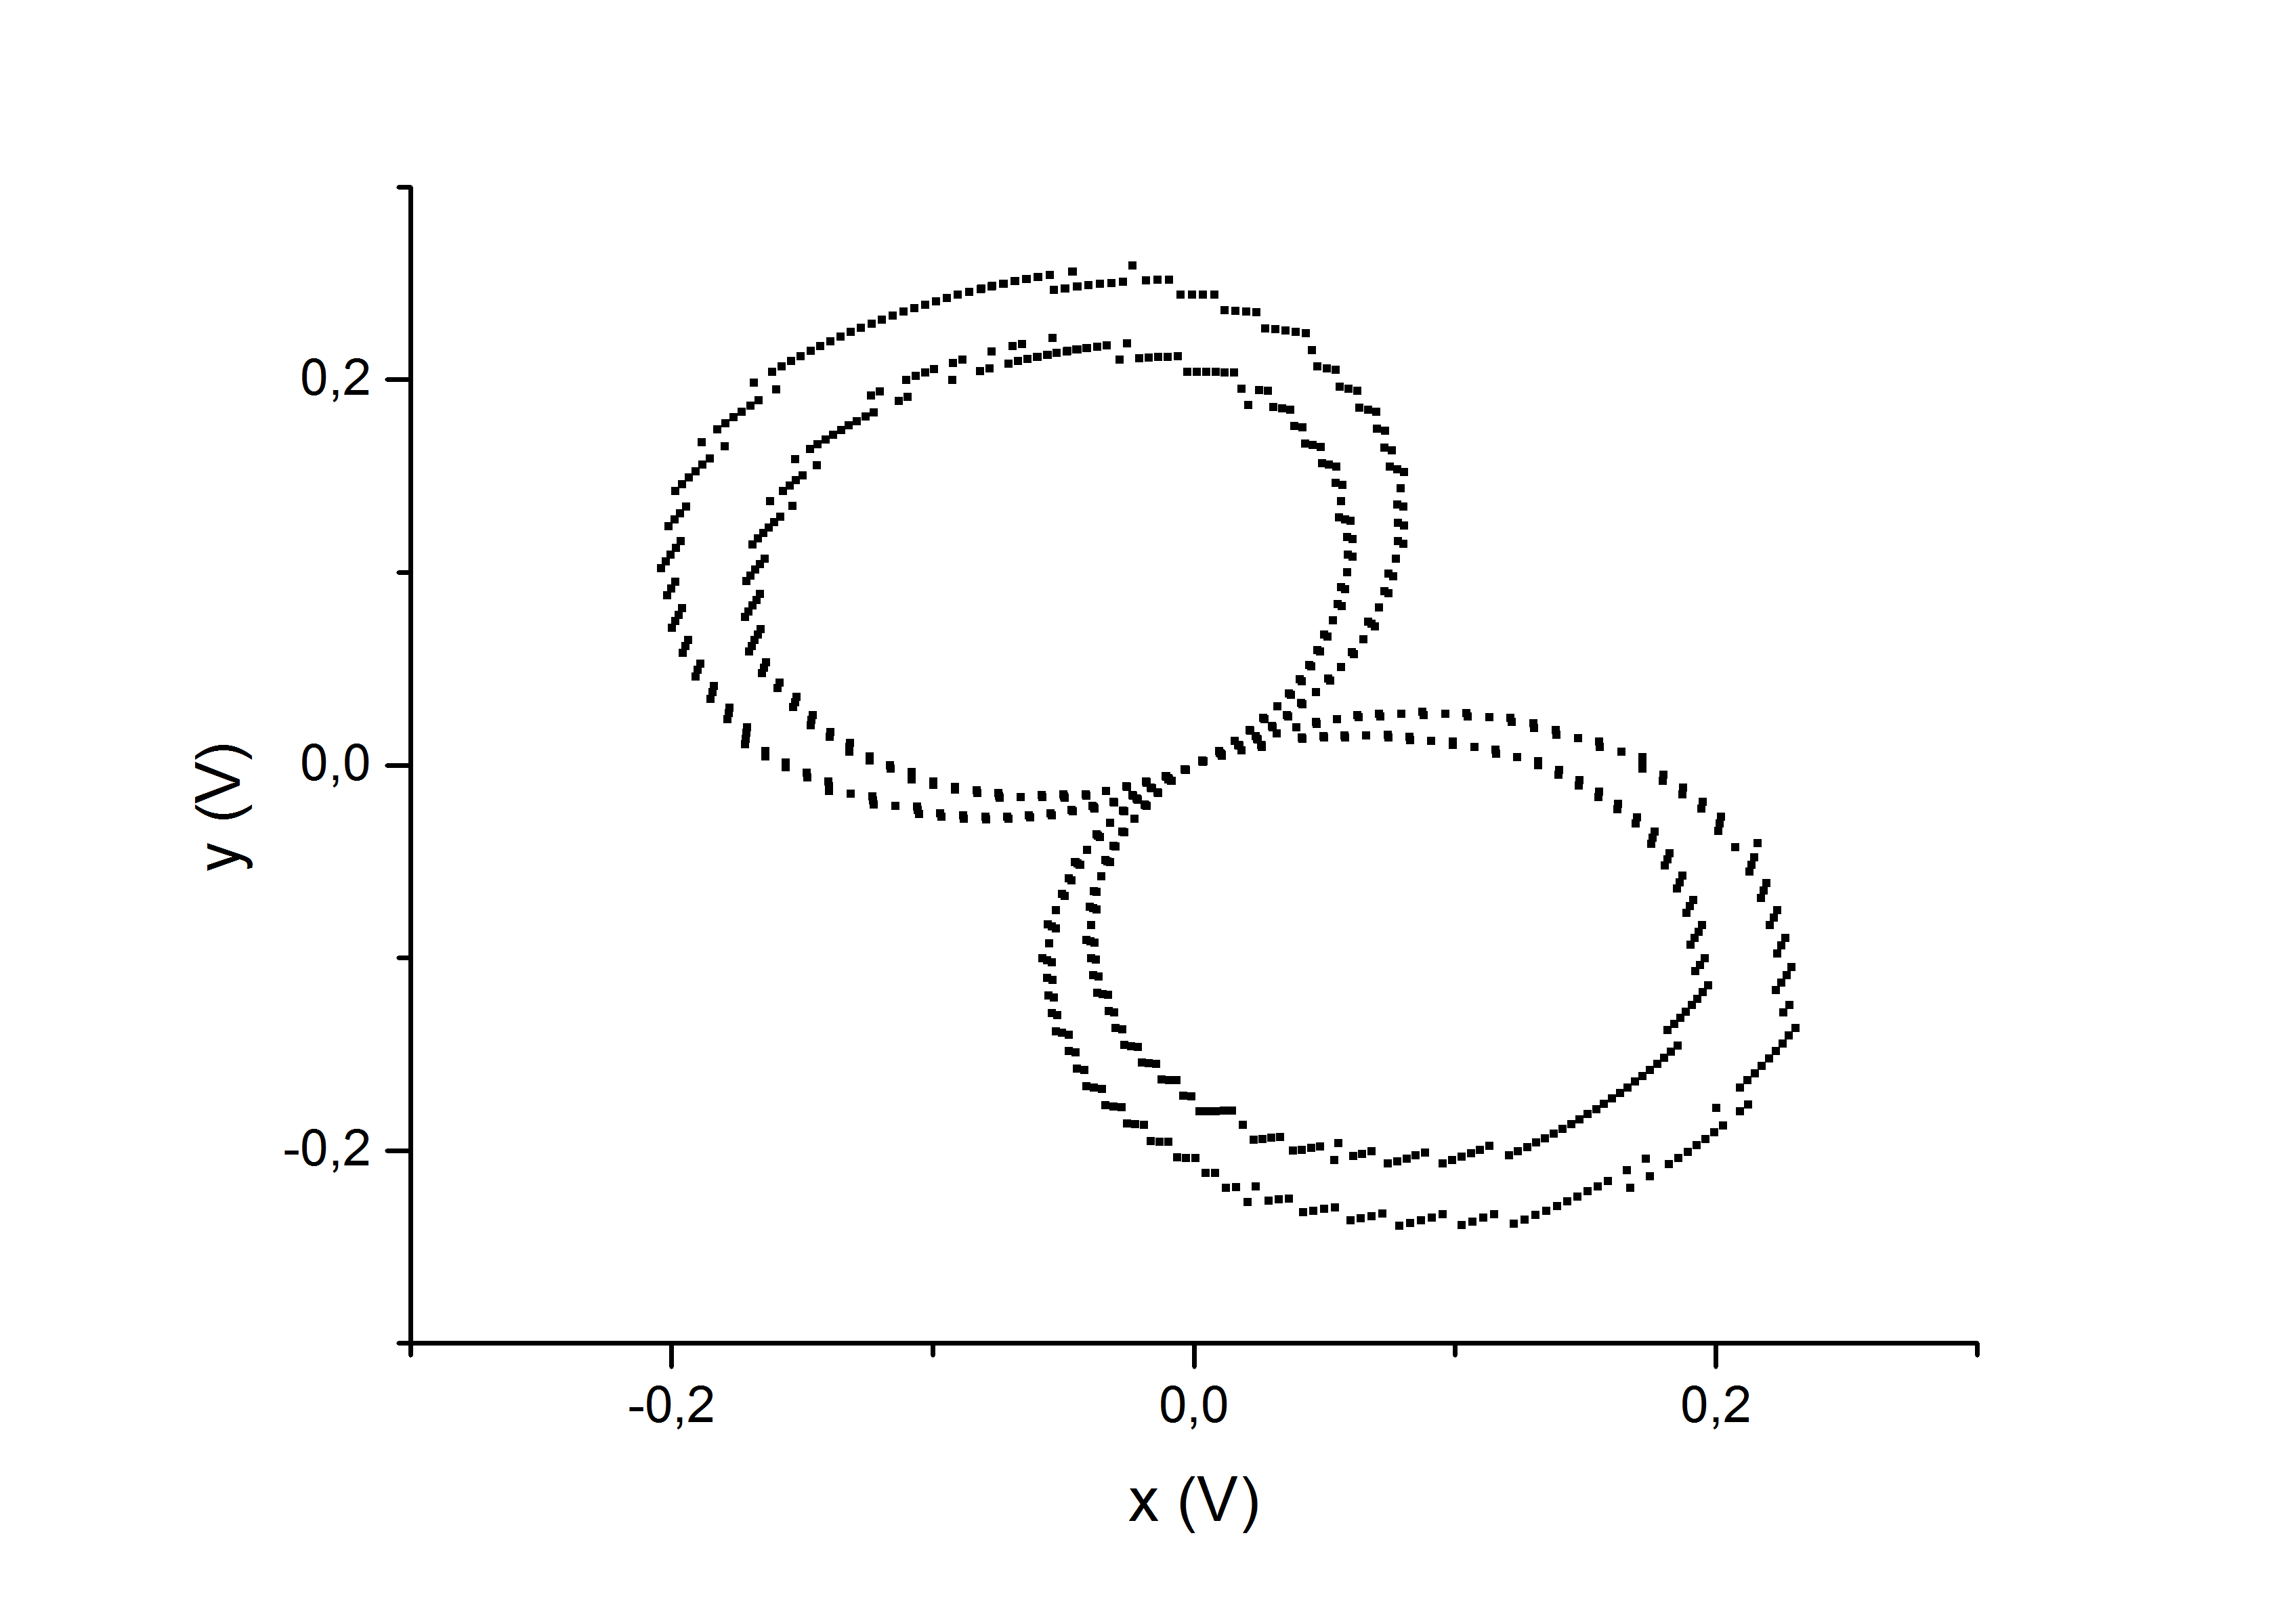
\includegraphics[scale=0.6]{Bilder/pw2}
\caption{Polarplot mit Widerstand R2}
\end{center}
\end{figure}
\begin{figure}[h]
\begin{center}
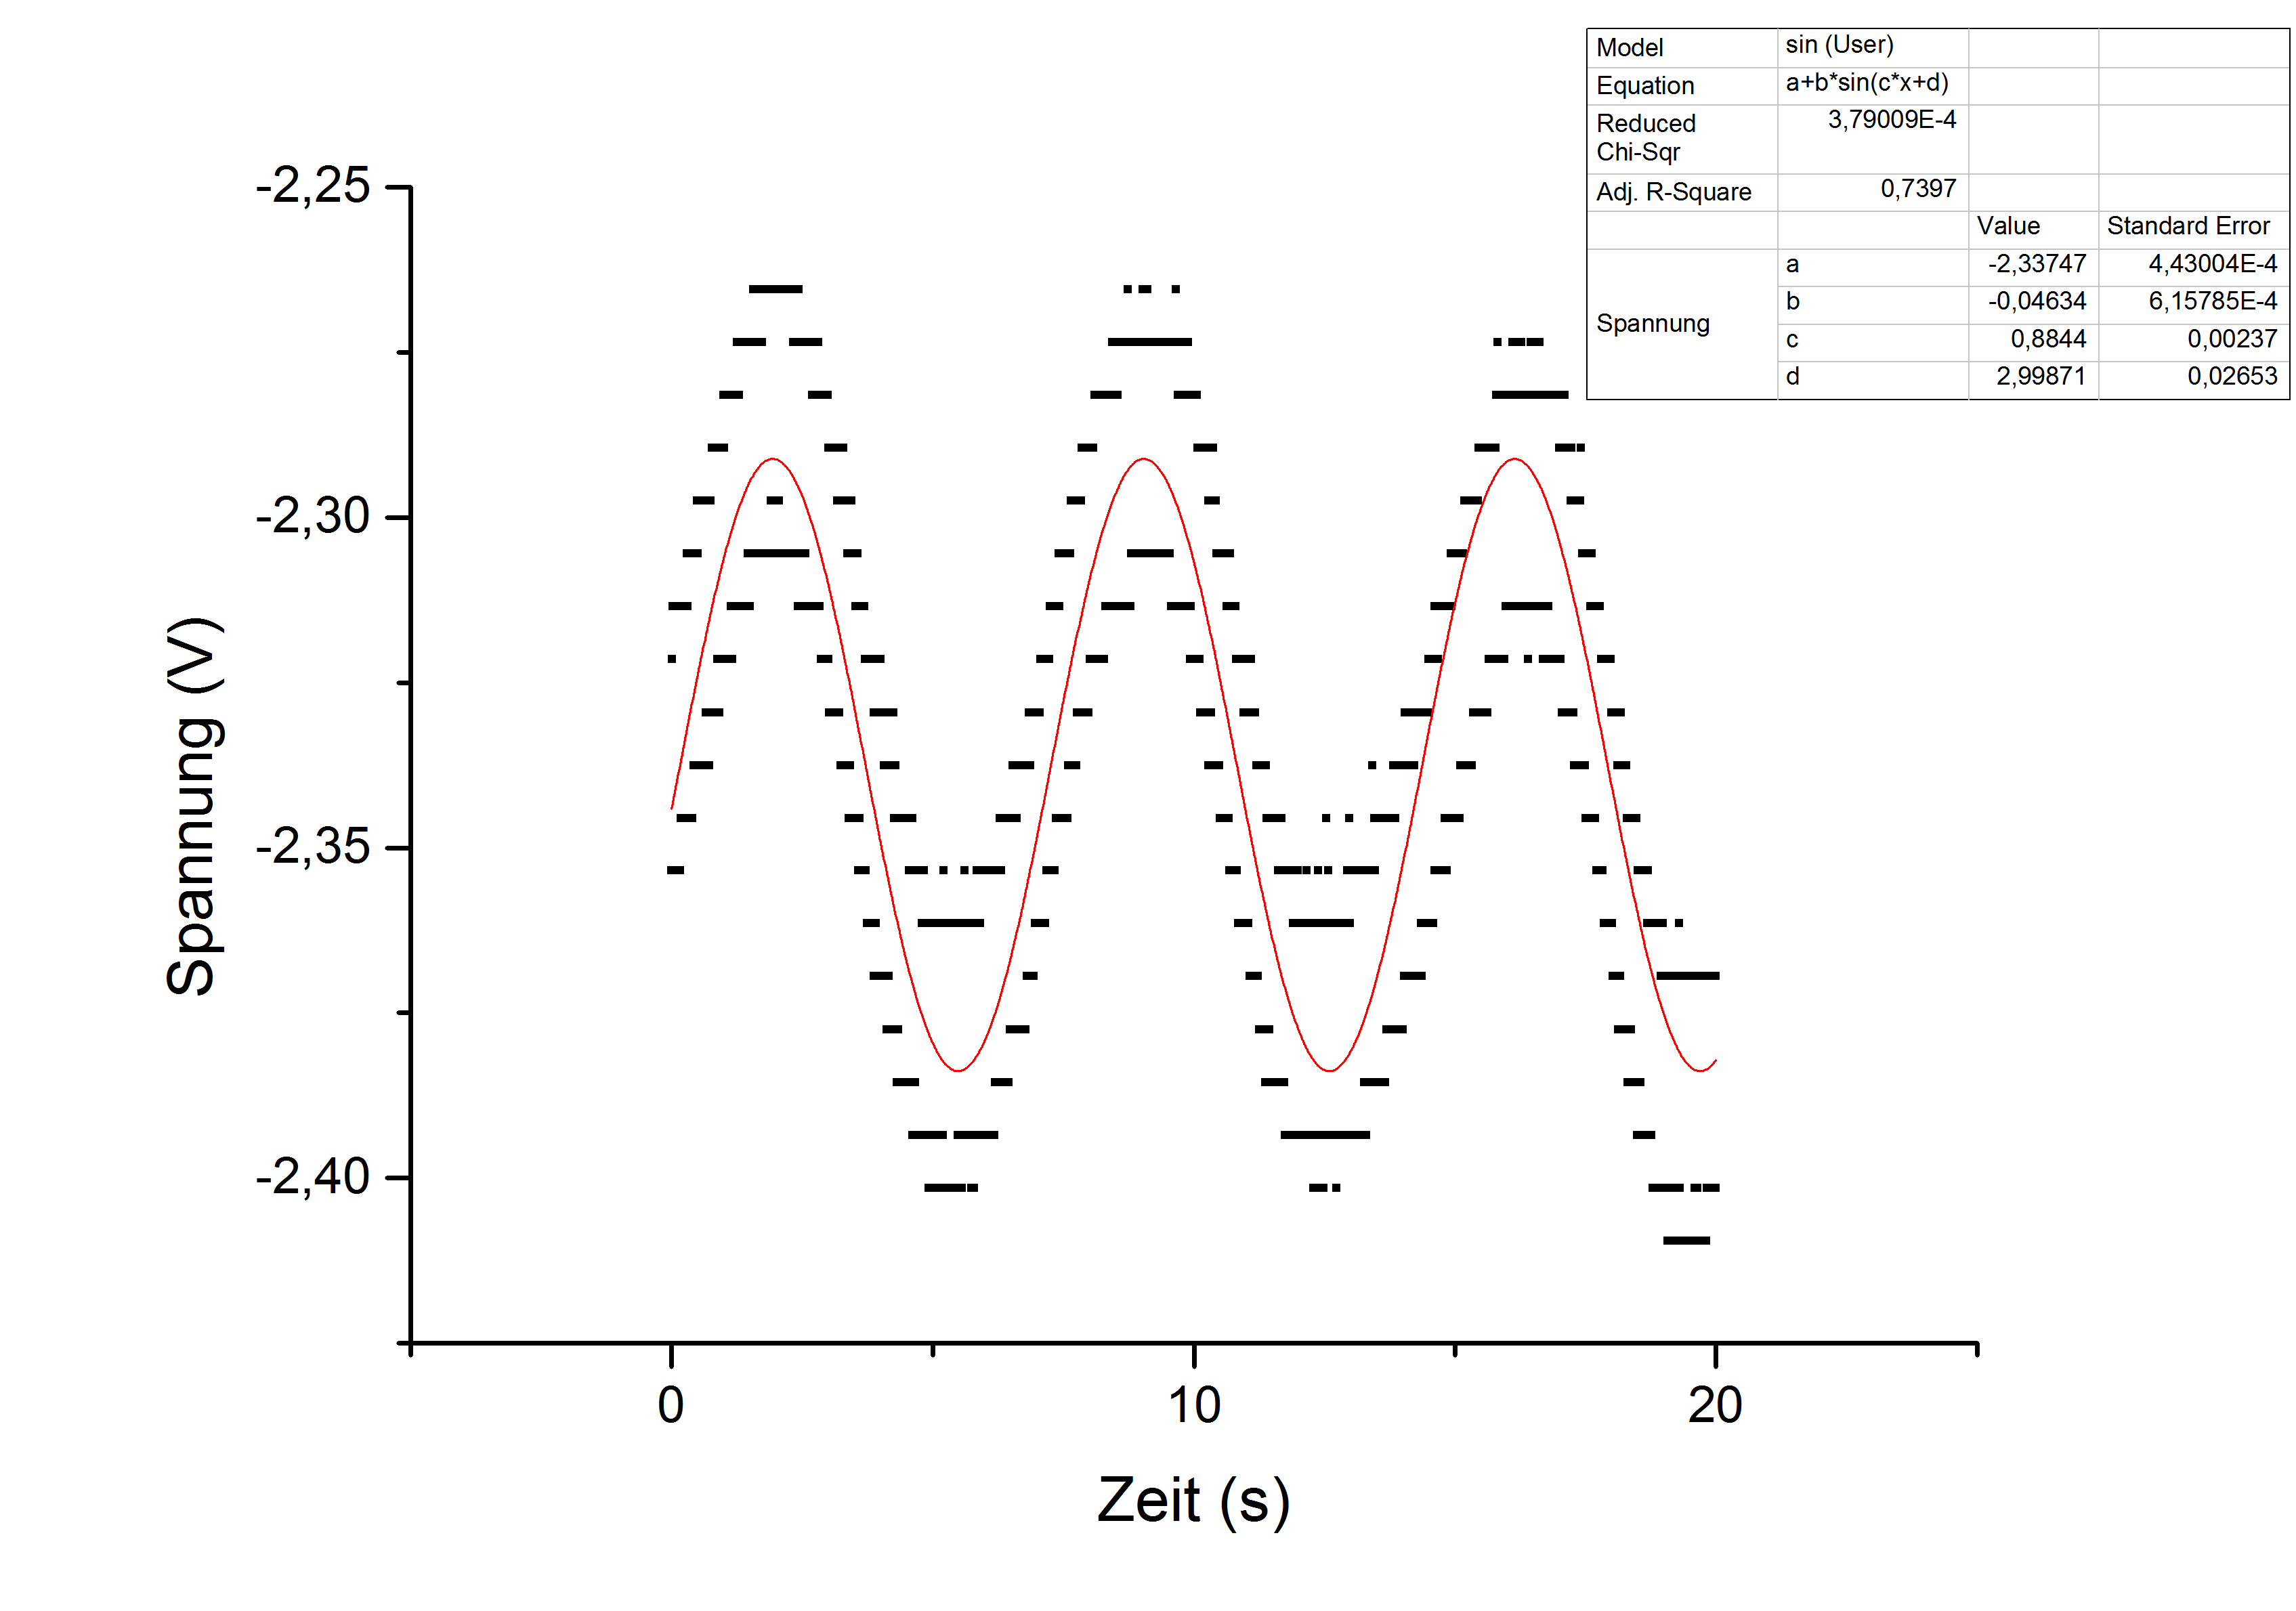
\includegraphics[scale=0.6]{Bilder/w3}
\caption{Messung mit Widerstand R3}
\end{center}
\end{figure}
\begin{figure}[h]
\begin{center}
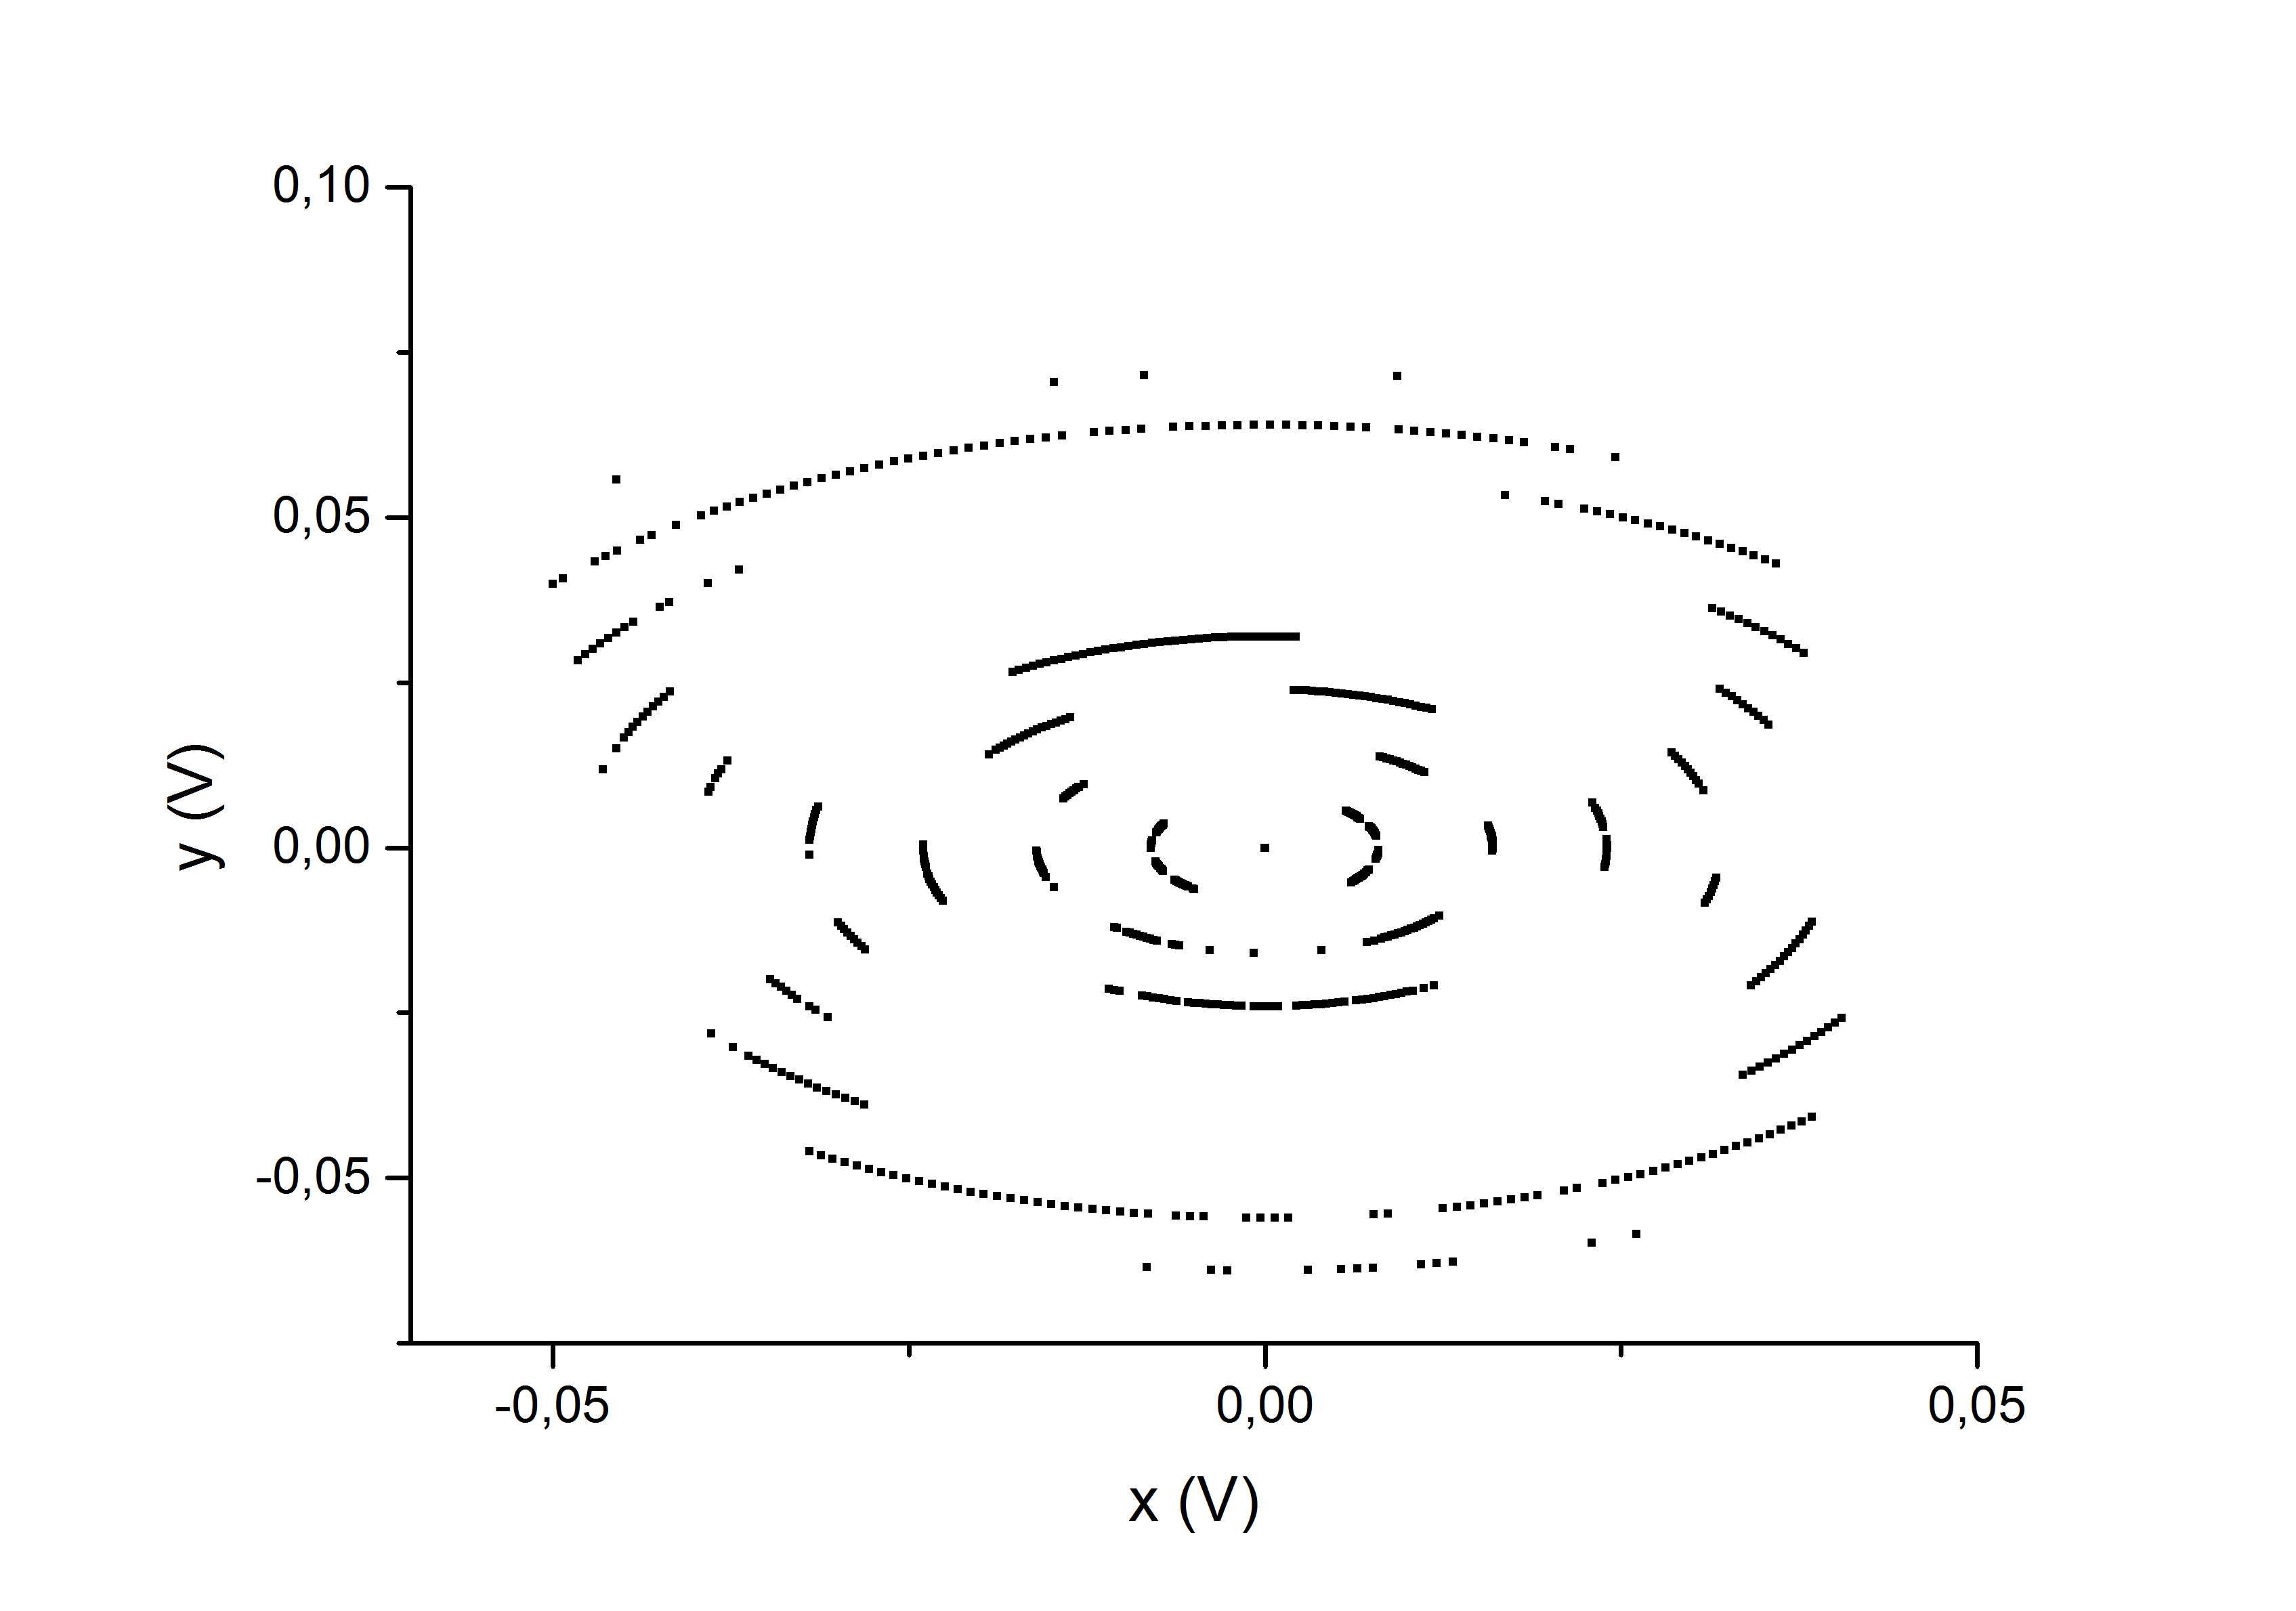
\includegraphics[scale=0.6]{Bilder/pw3}
\caption{Polarplot mit Widerstand R3}
\end{center}
\end{figure}
\begin{figure}[h]
\begin{center}
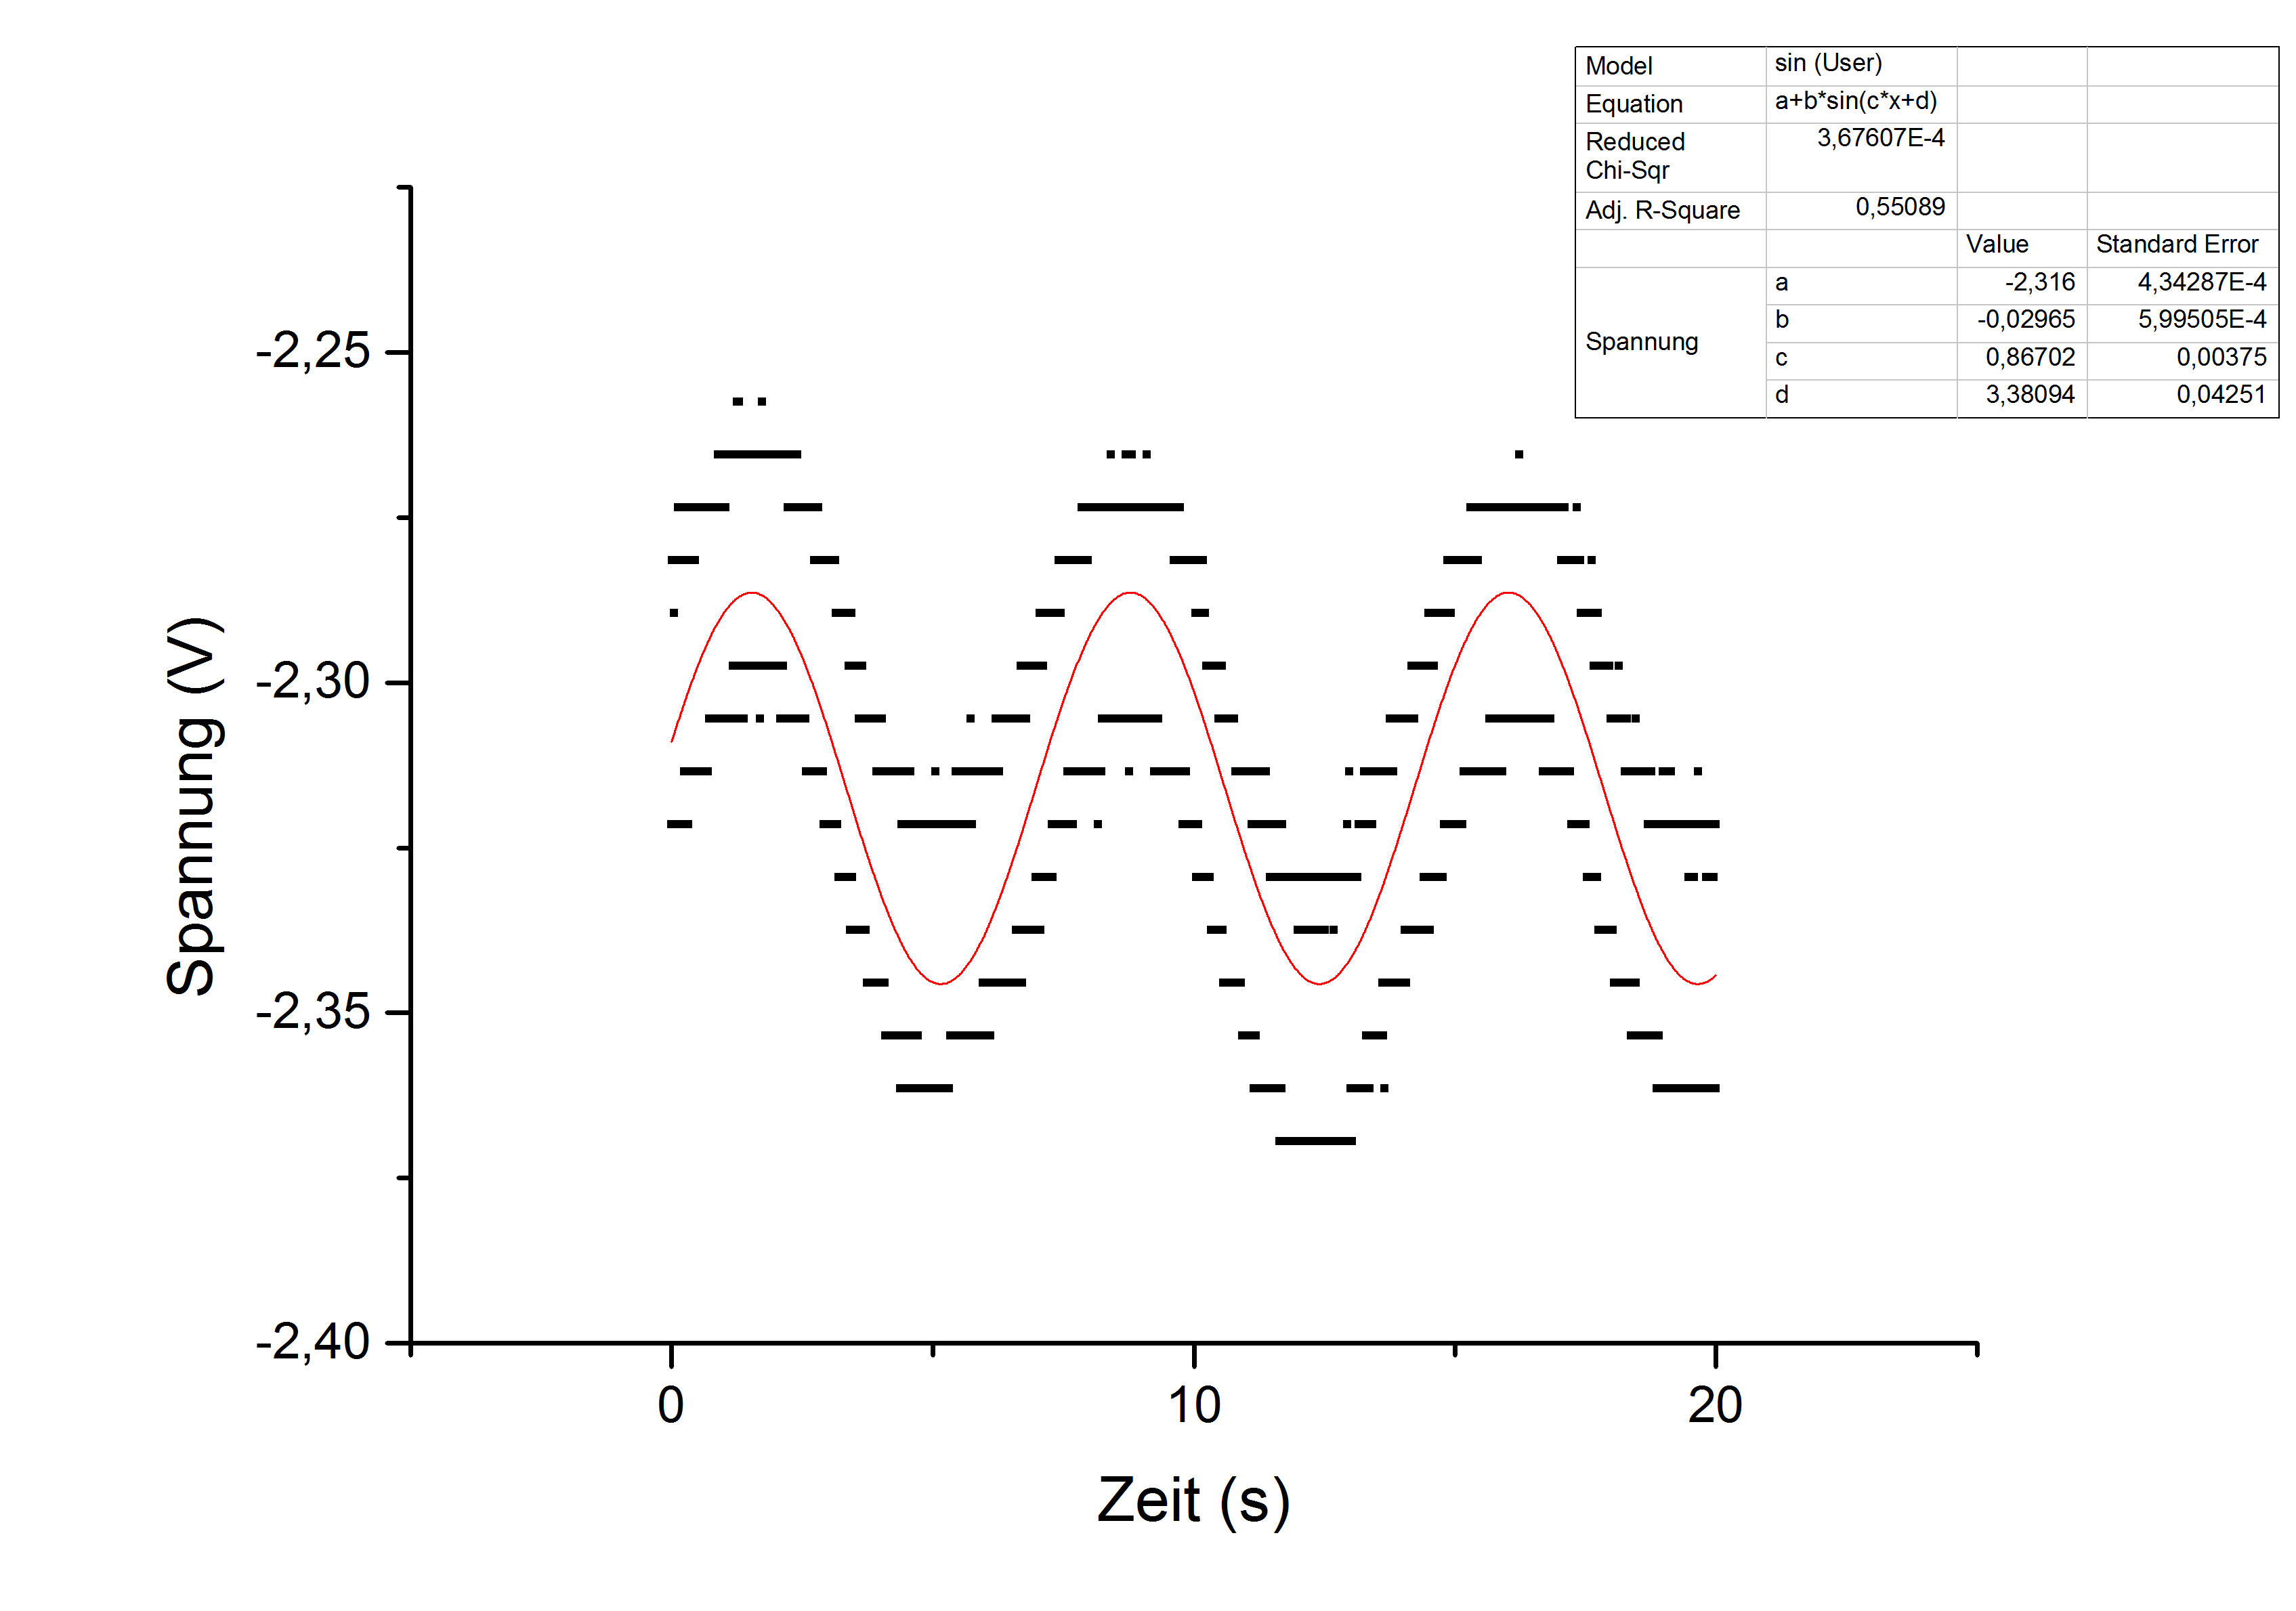
\includegraphics[scale=0.6]{Bilder/w4}
\caption{Messung mit Widerstand R4}
\end{center}
\end{figure}
\begin{figure}[h]
\begin{center}
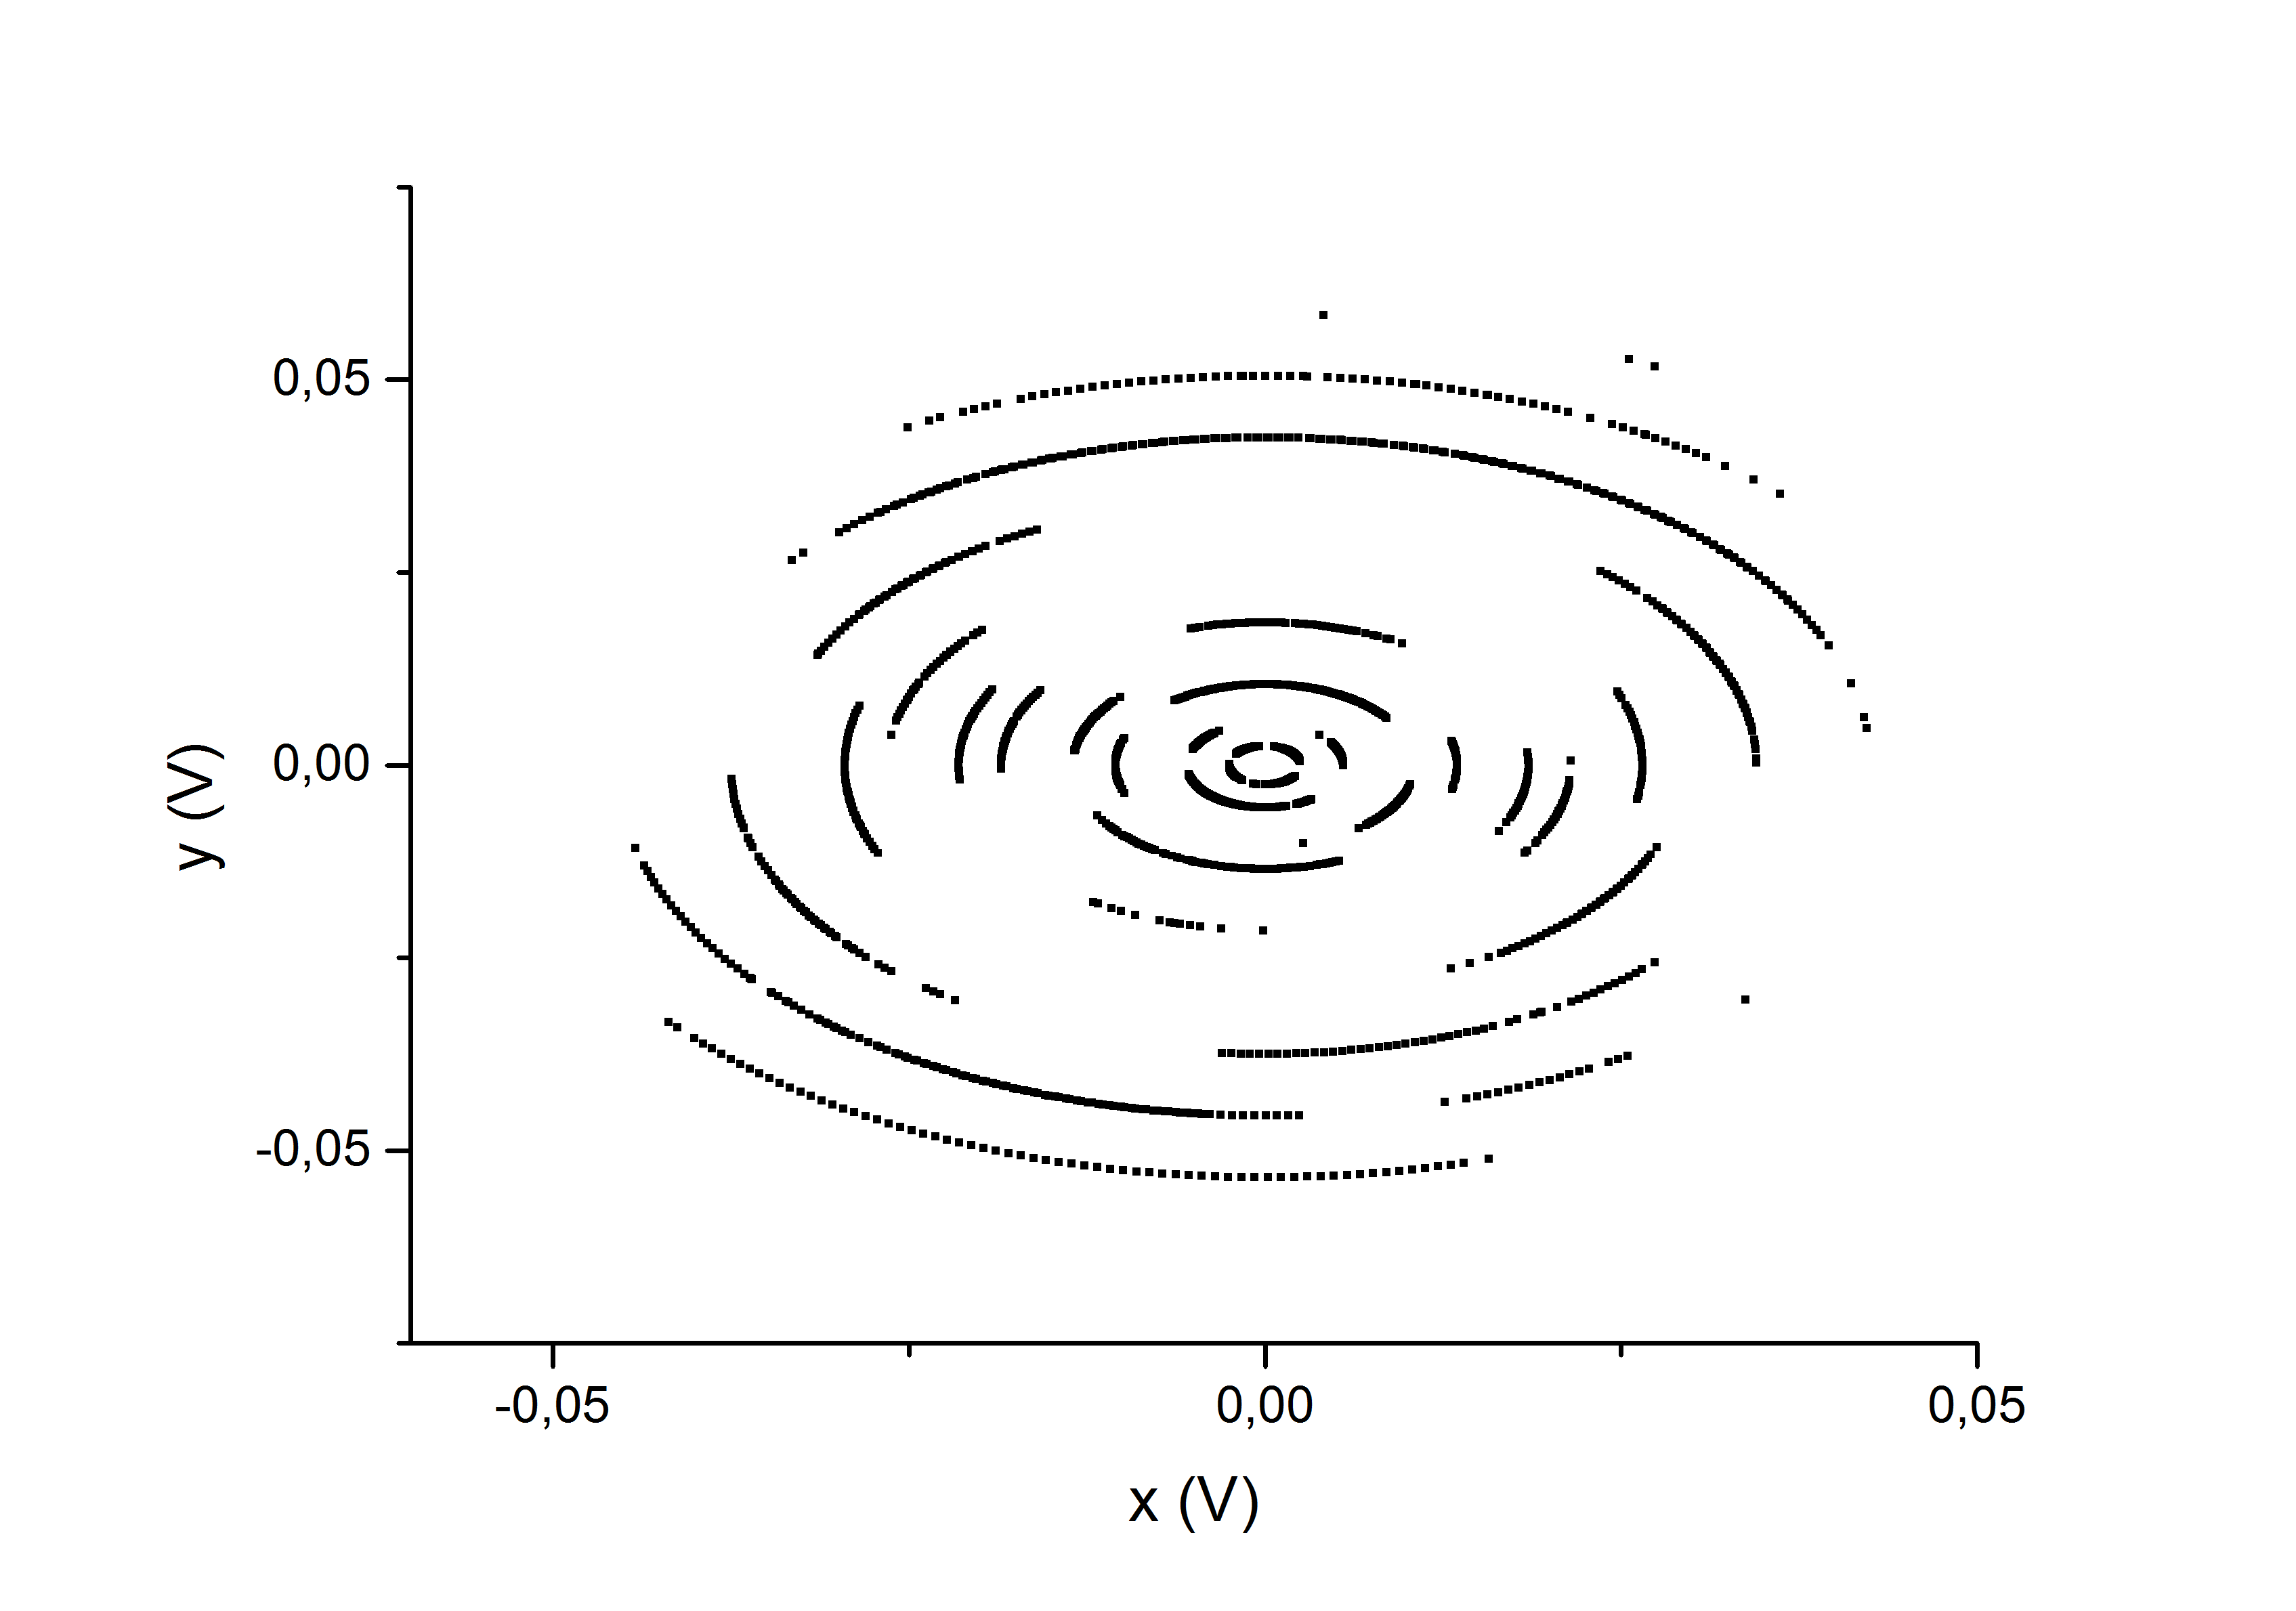
\includegraphics[scale=0.6]{Bilder/pw4}
\caption{Polarplot mit Widerstand R4}
\end{center}
\end{figure}
\begin{figure}[h]
\begin{center}
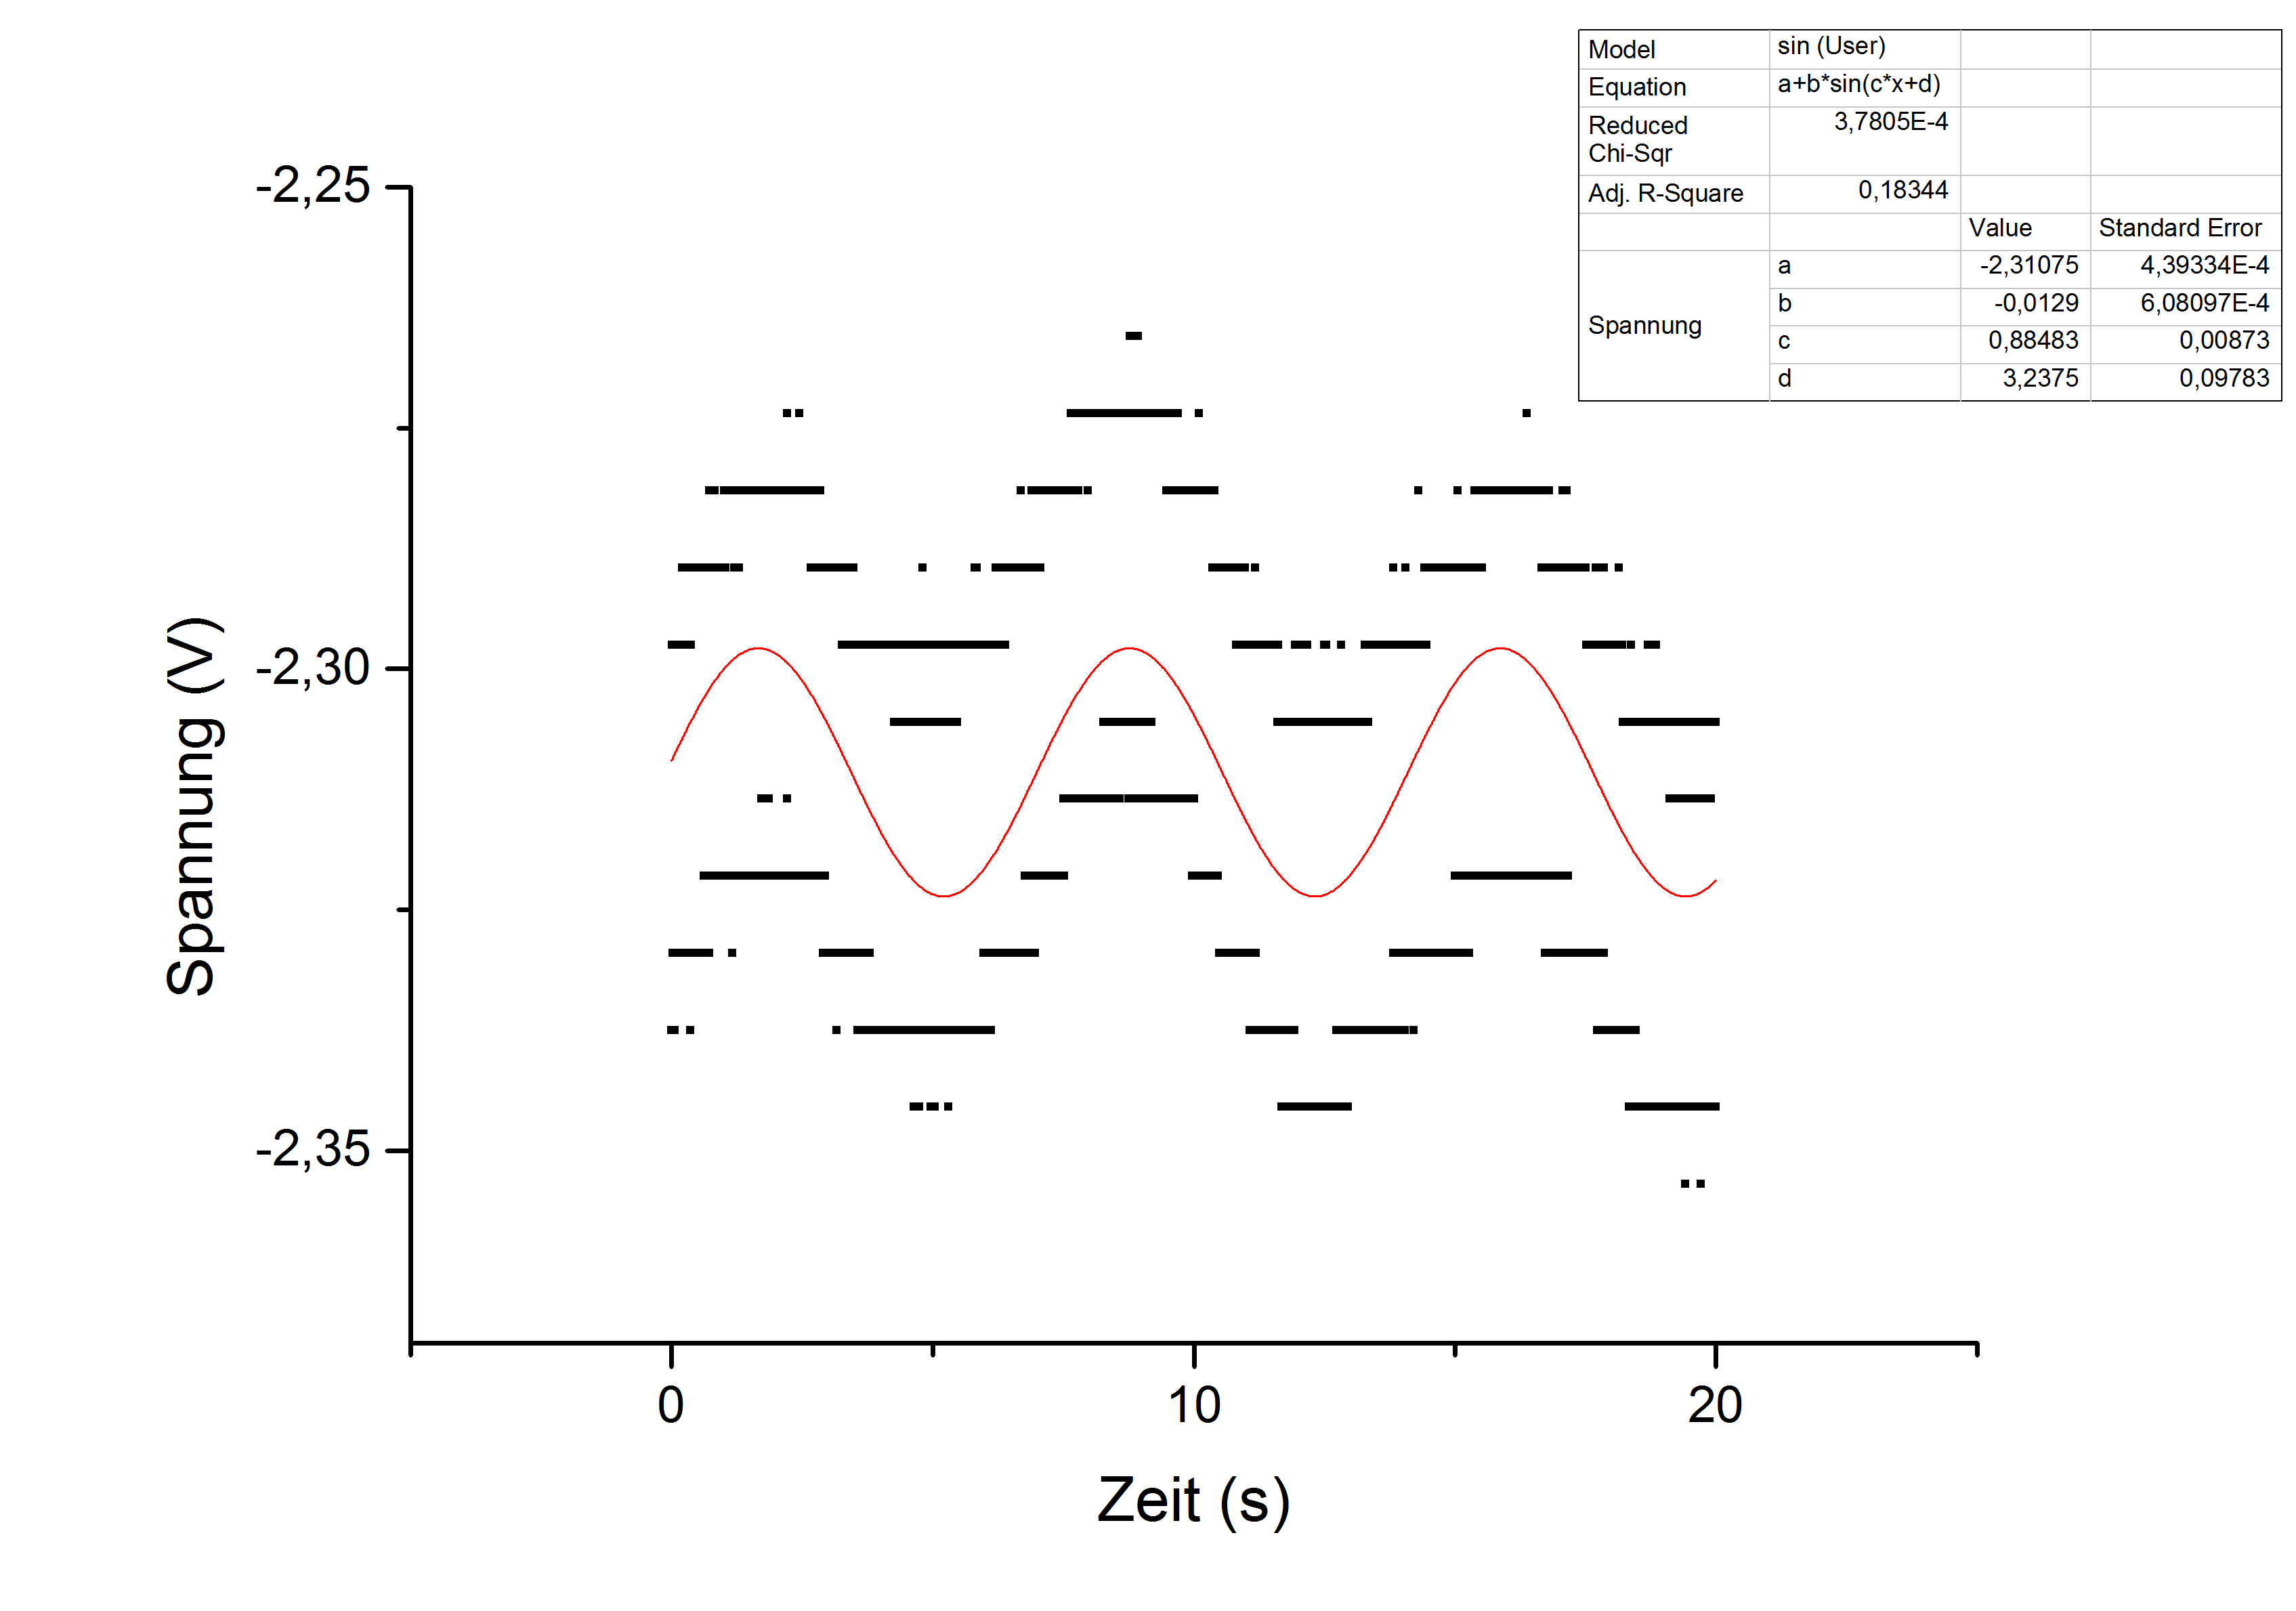
\includegraphics[scale=0.6]{Bilder/w5}
\caption{Messung mit Widerstand R5}
\end{center}
\end{figure}
\begin{figure}[h]
\begin{center}
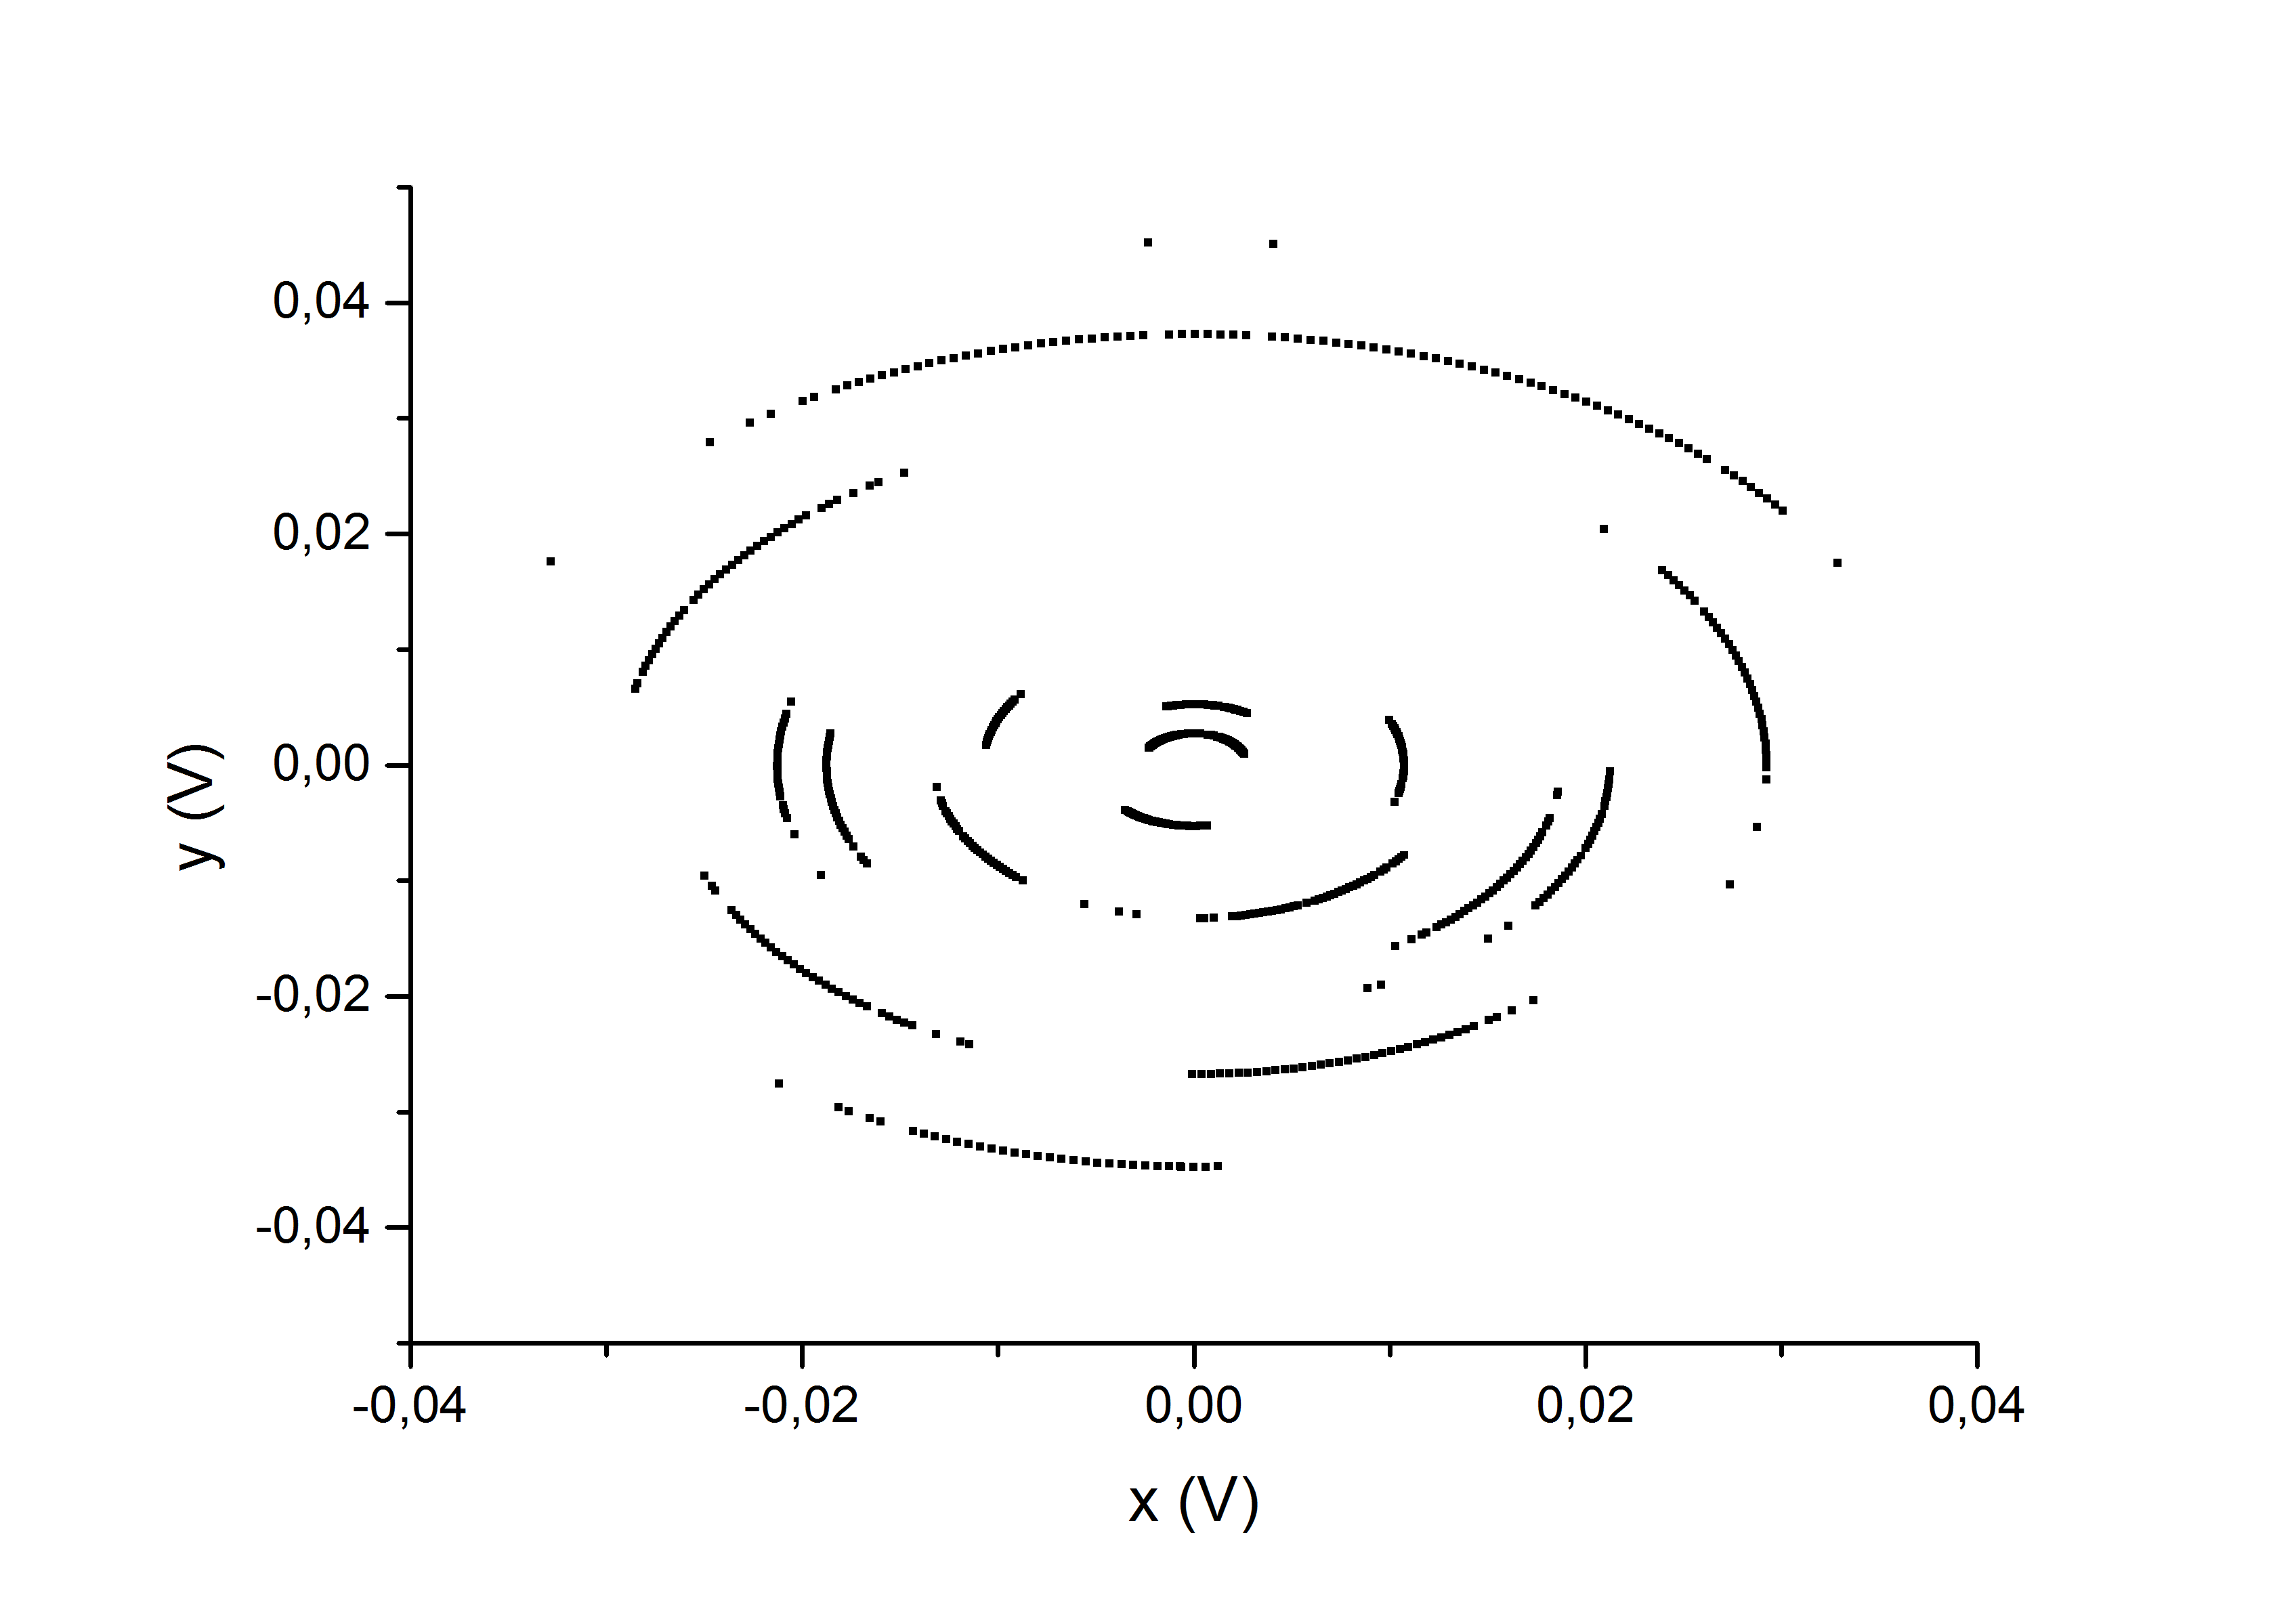
\includegraphics[scale=0.6]{Bilder/pw5}
\caption{Polarplot mit Widerstand R5}
\end{center}
\end{figure}
\begin{figure}[h]
\begin{center}
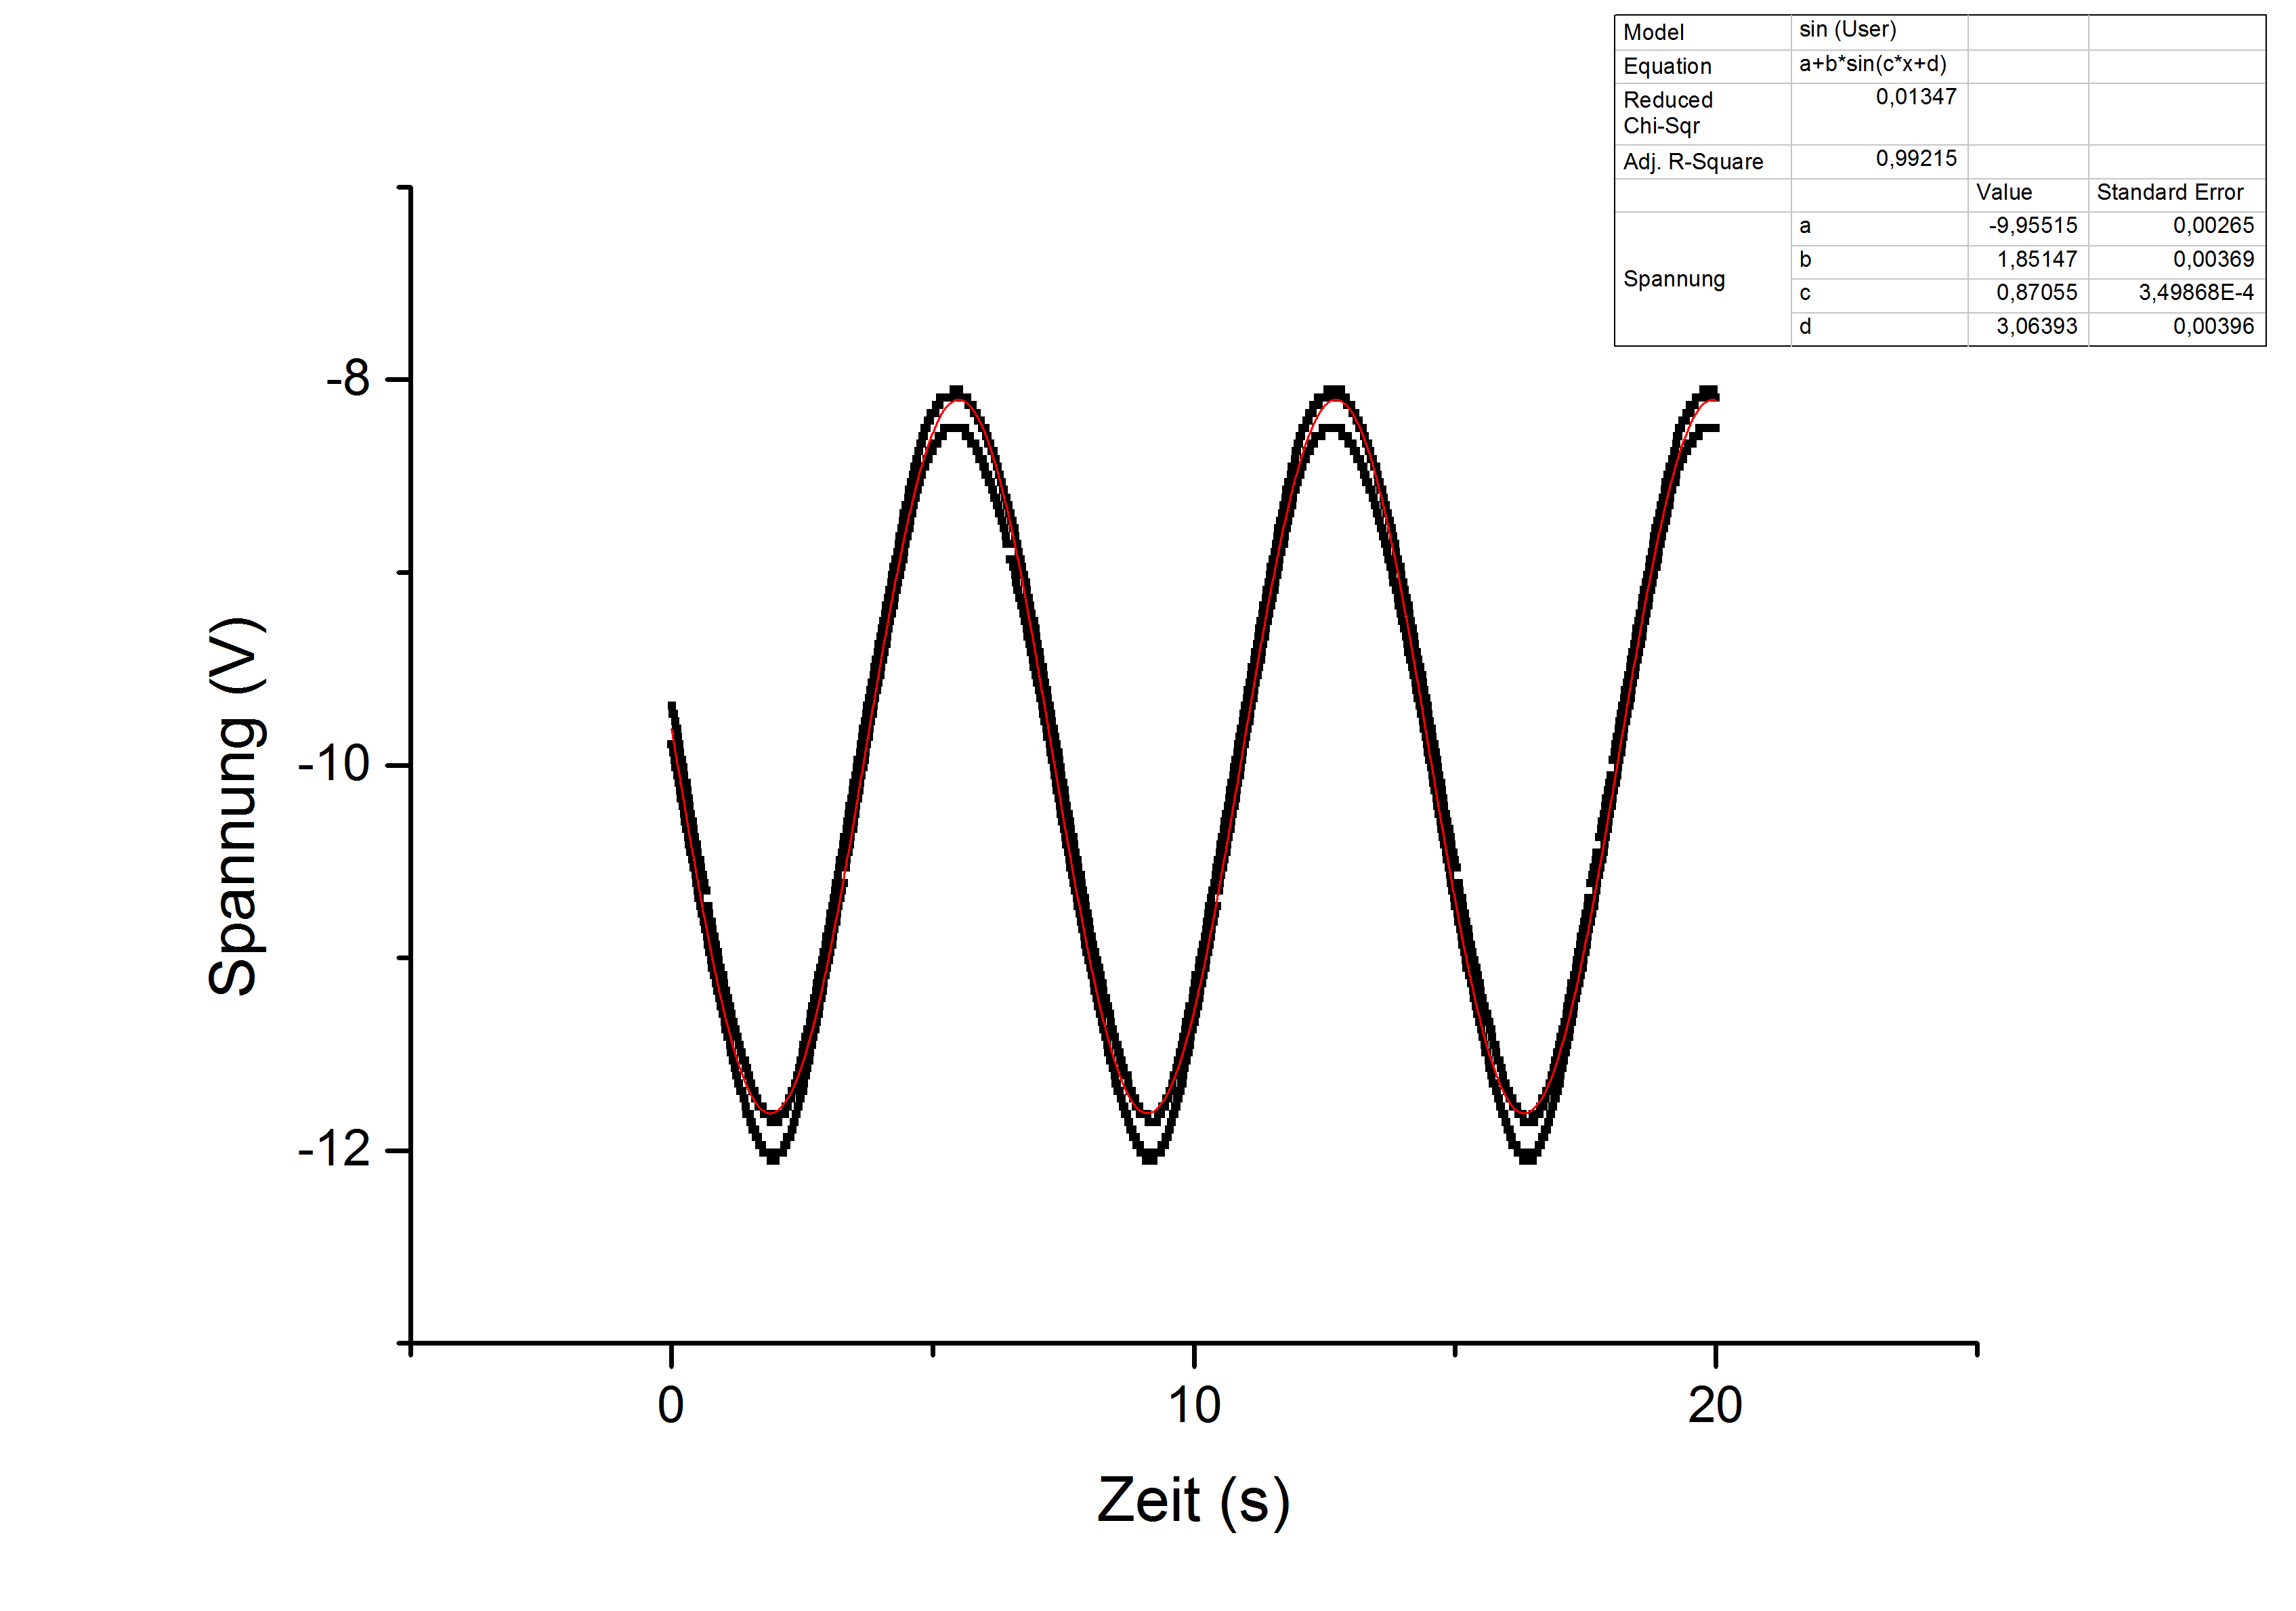
\includegraphics[scale=0.6]{Bilder/m1}
\caption{Messung mit Magnetospan}
\end{center}
\end{figure}
\begin{figure}[h]
\begin{center}
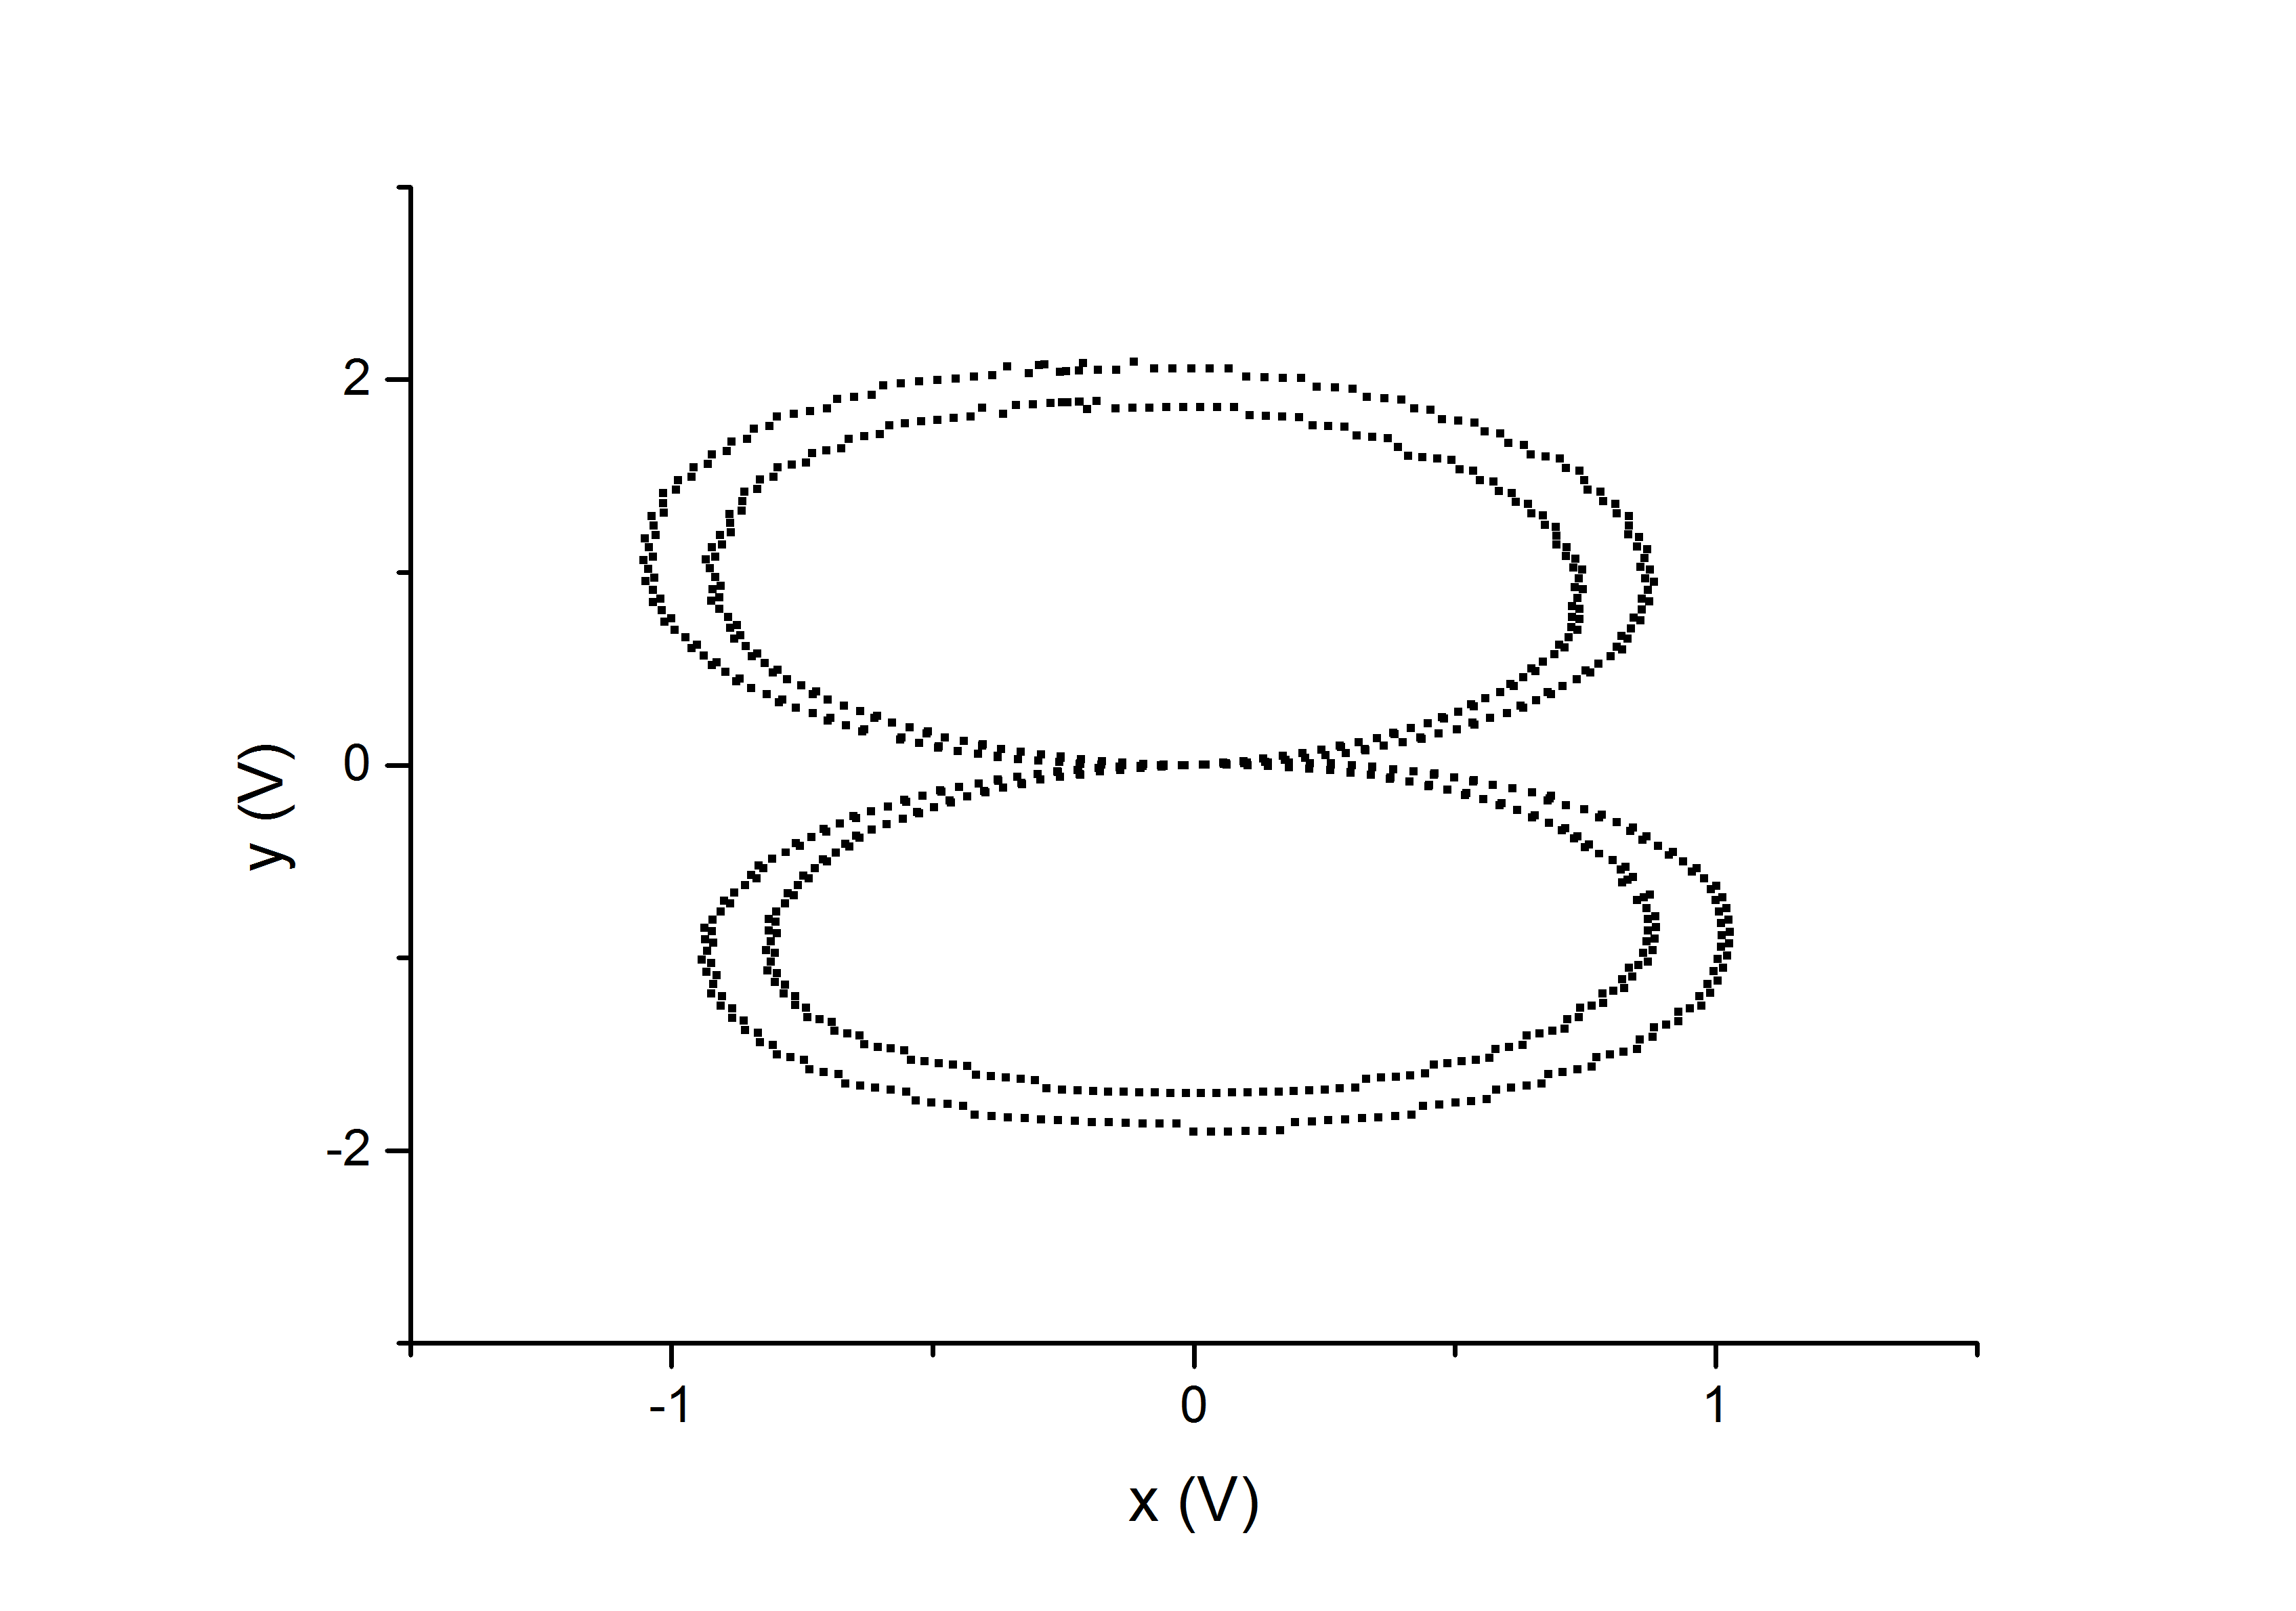
\includegraphics[scale=0.6]{Bilder/pm1}
\caption{Polarplot mit dem Magnetospan}
\end{center}
\end{figure}